\documentclass[notitlepage,reqno]{amsart}
% Packages I'm using
\usepackage{amsmath,amsfonts,amsthm,amssymb}
\usepackage{bbm}
\usepackage{cite}
%\usepackage{fullpage}
\usepackage{enumerate}
\usepackage[font=small,labelfont=bf]{caption}
\usepackage{framed}
\usepackage{setspace}
\usepackage{fancyhdr}
\usepackage{graphicx}
\usepackage{fancyvrb}
\usepackage{color}
\usepackage{listings}

% listings package parameters
\definecolor{javared}{rgb}{0.6,0,0} % for strings
\definecolor{javagreen}{rgb}{0.25,0.5,0.35} % comments
\definecolor{javapurple}{rgb}{0.5,0,0.35} % keywords
\definecolor{javadocblue}{rgb}{0.25,0.35,0.75} % javadoc

\lstset{
  language=Java,
  numbers=left,
  numbersep=7pt,
  basicstyle=\ttfamily\small,
  keywordstyle=\color{javapurple}\bfseries,
  stringstyle=\color{javared},
  commentstyle=\color{javagreen},
  morecomment=[s][\color{javadocblue}]{/**}{*/},
  numberstyle=\tiny\color{black},
  stepnumber=1,
  tabsize=2,
%  showspaces=false,
%  showstringspaces=false,
  breaklines=true
}

% Homework-specific information
\newcommand{\hmwkTitle}{Evolutionary Games on the Lattice}
\newcommand{\hmwkAuthor}{Andrea Sannier}
%\newcommand{\hmwkSubTitle}{}n
%\newcommand{\hmwkDueDate}{}
\newcommand{\hmwkClass}{Honors Thesis}
\newcommand{\hmwkClassTime}{}
\newcommand{\hmwkInstructor}{Dr. Nicolas Lanchier}


% Commonly-used stuff
\newcommand{\pr}{\mathbb{P}}
\newcommand{\E}{\mathbb{E}}
\newcommand{\R}{\mathbb{R}}
\newcommand{\N}{\mathbb{N}}
\newcommand{\seqx}{\{x_n\}_{n=0}^\infty}
\newcommand{\seqy}{\{y_n\}_{n=0}^\infty}
\newcommand{\seqa}{\{a_n\}_{n=0}^\infty}
\newcommand{\seqb}{\{b_n\}_{n=0}^\infty}

% Allowing easy statement of theorems and lemmas (requires amsthm)
\newtheoremstyle{normal}
	{3pt}			%space above
	{3pt}			%space below
	{}				%body font
	{\parindent}	%indent amount
	{\itshape}		%theorem head font
	{}				%punctuation after theorem head
	{ }		%space after theorem head
	{}				%theorem head specification(??)
\newtheorem{thm}{Theorem}
\newtheorem*{thm*}{Theorem}
\newtheorem{lem}{Lemma}
\newtheorem*{lem*}{Lemma}

% Margins and other formatting
%\topmargin=0in
%\leftmargin=-1in
%\rightmargin=-1in
\setlength{\parindent}{.25in}
\fvset{xleftmargin=2em}		%fancyvrb package allows indentation of all Verbatim environments

% Simple environment to change margins around the Abstract section
\newenvironment{changemargin}[2]{
\begin{list}{}{
\setlength{\topsep}{0pt}
\setlength{\leftmargin}{#1}
\setlength{\rightmargin}{#2}
\setlength{\parindent}{0 pt}
\setlength{\listparindent}{\parindent}
\setlength{\itemindent}{\parindent}
\setlength{\parsep}{\parskip}
}
\item[]}{\end{list}}

% Setup the header and footer
\pagestyle{fancy}
\pagenumbering{arabic}

\lhead{}
\chead{\hmwkTitle}
\rhead{\hmwkAuthor}
\cfoot{\thepage}
\addtolength{\headheight}{12pt}
\setlength{\headsep}{0.125in}
\setlength{\footskip}{0.75in}
\renewcommand\headrulewidth{0.4pt}
\renewcommand\footrulewidth{0pt}

%%%%%%%%%%%%%%%%%%%%%%%%%%%%%%%%%%%%%%%%%
% Make Title
\title{\huge{\textmd{\textbf{\hmwkTitle}}}}
\date{}
\author{\textbf{\hmwkAuthor} \\
\textmd{First Reader: \hmwkInstructor}}
%%%%%%%%%%%%%%%%%%%%%%%%%%%%%%%%%%%%%%%%%

\begin{document}

\maketitle
\thispagestyle{fancy}

\begin{changemargin}{.3in}{.3in}
\section*{Abstract}
Traditionally, models in evolutionary game theory are based on mean-field
ordinary differential equations and, therefore, on a central
assumption that players are well-mixing, i.e., that any two players may interact with equal probability. This thesis intends to shed light
on a way to avoid making this assumption by re-imagining the models to
account for space and stochasticity. We place countably many players
on an infinite $d$-dimensional lattice and allow them to play games
only with some set of neighbors. Moreover, the games they
play are not deterministic and are instead governed by one of seven
stochastic processes that depend on the fitnesses of the neighboring
players. Using computer simulations of these processes, we discover a number of surprising results that differ from those found in traditional models, perhaps most notably that, in some prisoner's dilemma situations, cooperation is the most effective strategy.
\end{changemargin}

\section{Introduction: What is Game Theory?}
\subsection{Definition}
Game theory is the mathematical modeling of situations in which
individuals compete for a desirable outcome with each player's
outcome dependent upon the choices made by her competitors. As with
any model, a number of assumptions are required, certainly not the
least of which is the assumption that the players behave rationally. A
game as a mathematical object comprises a set of players, a set of
strategies those players may employ, and a way to map choice of
strategy to some payoff. In this thesis, the last of these will be accomplished by use of a payoff matrix, which will be defined below. With just these three simple elements, we gain a great deal of insight into many systems involving interacting humans, animals, and computers.

\subsection{Johns von Neumann and Nash}
John von Neumann is by most accounts the inventor of game theory, and is certainly responsible for its mathematical rigor. Known as one of the greatest minds of his (or any) time\cite{glimm}, von Neumann did foundational work in an incredible number of fields, perhaps the most well-known of which are computer science, quantum mechanics, nuclear physics, and, of course, game theory. Von Neumann's contribution to game theory began in 1928 with the publication of his minimax theorem, which is a key result for two-person, zero sum games (games in which positive payoffs for one player correspond to equal negative payoffs for the other, so the net payoff is always zero). In this theorem, von Neumann established the concept of an optimal strategy, which is one that minimizes the maximum negative payoff, and is a key stepping-stone on the road to the famous Nash equilibrium, which is one kind of optimal strategy. Beyond this important result, von Neumann also co-authored with Oskar Morgenstern what is generally considered to be the seminal text on the subject of game theory: \emph{Theory of Games and Economic Behavior}\cite{vonNeumann}. In it, the authors outline a rigorous mathematical definition of games and, probably due to the influence of Morgenstern, an economist, detail how and when to apply these mathematical objects to the field of economics. 

Any discussion of game theory must also mention John Nash, for whom the aforementioned Nash equilibrium is named. Though he is perhaps more well-known today for his battle with schizophrenia (as depicted in the book and film \emph{A Beautiful Mind}), the work that won him a Nobel Prize in Economics was his development of the Nash equilibrium in 1950. It is worth noting that the first award he received for this discovery was the 1978 John von Neumann Theory Prize. The Nash equilibrium is a concept now central to game theory that describes a specific state a game may reach in which no player can gain in expected payoff by changing her strategy\cite{rubinstein}. We will see in a moment how these equilibria can be represented in a payoff matrix, but for now let it suffice to say that the Nash equilibrium is heavily studied, refined, and employed throughout applications of game theory.

\subsection{The payoff matrix}
\label{sec:payoffmatrix}
With this (admittedly cursory) historical background in hand, we can now better define the structures used in game theory models. Let $S$ be a set of $n$ strategies. Then we encode the relationship between competing strategies in an $n$-by-$n$ matrix
\[
    P = 
    \begin{pmatrix}
      a_{11} & a_{12} & \cdots & a_{1n} \\
      a_{21} & & & \\
      \vdots & & \ddots & \\
      a_{n1} & & & a_{nn}
    \end{pmatrix}.
\]

When a player, $A$, employs strategy $i$ against another player, $B$
using strategy $j$, $A$ receives a payoff of $a_{ij}$, and $B$
receives a payoff of $a_{ji}$. We see immediately that the concept of
payoff is well-defined; if any two players play a game using any
pairing of the $n$ strategies, each player will receive some payoff.

For a two-strategy game, we can easily define the Nash equilibrium
mentioned above.  Given a game defined by a payoff matrix
\[
    P =
    \begin{pmatrix}
      a_{11} & a_{12} \\
      a_{21} & a_{22}
    \end{pmatrix},
\]
we say that strategy 1 is a Nash equilibrium if $a_{11}\geq a_{21}$ (symmetrically, strategy 2 is a Nash equilibrium if $a_{22}\geq a_{12}$). We can see in the first case that if both players have already chosen strategy 1, both players will receive a payoff of $a_{11}$. If either is to unilaterally change to strategy 2, she will instead receive the at-best-as-desirable payoff of $a_{21}$. The symmetrical case in which $a_{22}\geq a_{12}$ shows the same behavior.

It is also worth spending some time to examine a famous type of game, the prisoner's dilemma. The following from the Stanford Encyclopedia of Philosophy is a standard setup for the problem\cite{stanford}:
\begin{quote}
Tanya and Cinque have been arrested for robbing the Hibernia Savings Bank and placed in separate isolation cells. Both care much more about their personal freedom than about the welfare of their accomplice. A clever prosecutor makes the following offer to each. ``You may choose to confess or remain silent. If you confess and your accomplice remains silent I will drop all charges against you and use your testimony to ensure that your accomplice does serious time. Likewise, if your accomplice confesses while you remain silent, they will go free while you do the time. If you both confess I get two convictions, but I'll see to it that you both get early parole. If you both remain silent, I'll have to settle for token sentences on firearms possession charges. If you wish to confess, you must leave a note with the jailer before my return tomorrow morning.''
\end{quote}

In this scenario, the optimal choice is always to confess, since
neither player knows the other's choice. It is in a sense socially
optimal for both players to confess, since the total payoff is
maximized this way, but maximum individual payoff can only be attained
by confessing while the other player remains silent. In this paper, we will use the terms
``cooperate'' and ``defect'' for ``remain silent'' and ``confess'',
respectively. In terms of a two-strategy payoff matrix: $a_{11}$
represents the ``token sentence'' payoff, $a_{12}$ the ``serious
time'' payoff, $a_{21}$ the ``freedom'' payoff, and $a_{22}$ the
``parole'' payoff. Thus, the game is simply a two-strategy payoff
matrix with $a_{21} > a_{11} > a_{22} > a_{12}$. Indeed, this
coefficient ordering defines the two-player prisoner's dilemma in the absence of the anecdotal setup. We will see later in this paper that traditional analysis of these games gives a significantly different result from the spatial and stochastic model.

\section{Evolutionary Game Theory}
\subsection{Definition}
Evolutionary game theory (EGT) is, as the name suggests, a restriction
of the field of game theory. In EGT, there is no rationality
assumption; a given player may possess only a single, unchanging
strategy. A player's payoff determines her fitness, and this fitness is
dependent on the relative proportions of the strategies in some
population. In this way, EGT is better-equipped than pure game theory
to model a number of biological systems such as predator-prey
competitions (since a rabbit cannot change its strategy to become a
wolf) and evolutionary systems (since nothing can change its own
phenotype). It is also assumed that players interact in a random,
proportion-dependent fashion. Since higher payoffs are associated with
greater fitness, we interpret success in a game as evidence of
reproductive success; over time, strategies that perform well
(i.e., receive more payoff, which corresponds to greater fitness)
will out-reproduce poorer strategies.

In general, EGT models are formed based on the central assumption that
players are well-mixing, i.e., that any player can play with any
other with equal probability. In
this thesis, however, we eliminate this assumption by accounting for interactions in
space with each interaction governed by a stochastic process. We
place players on a $d$-dimensional grid and, rather than allowing
well-mixing interactions, we allow players to compete only with some
neighborhood along the $d$ dimensions. Moreover, interactions are
non-deterministic; a player's fitness speaks only to a probability of
victory rather than determining outright who is left standing after the game.

\subsection{John Maynard Smith}
If ever there has been a field whose existence can be attributed to a
single person, it is evolutionary game theory, and that person is John
Maynard Smith, a British evolutionary biologist. Maynard Smith was the
first to apply game theory to his branch of biology, where it now flourishes,
illuminating a great many human and animal phenomena. Maynard Smith's
work on EGT began in 1973, when he published a paper in
\emph{Nature} outlining his concept of an evolutionarily stable
strategy (ESS), which is similar to the Nash equilibrium (though
Maynard Smith was unaware of Nash's work when developing the ESS).
A strategy is an ESS if it cannot be overtaken by a competing strategy
with very small initial proportion (that is, given an infinite
population of the ESS strategy, an infinitesimal group of invaders
will be eliminated). We can also define an ESS in terms
of a payoff matrix; recall the form
\[
    P = 
\begin{pmatrix}
  a_{11} & a_{12} \\
  a_{21} & a_{22}
\end{pmatrix}.
\]

A strategy has the ESS property if either (i) $a_{11} > a_{21}$ or
(ii) $a_{11} = a_{21}$ and $a_{12} > a_{22}$.

Maynard Smith's contributions to his field did not stop there, though;
in 1982, he published a book called \emph{Evolution and the Theory of
  Games}, which, while still most famous for fleshing out the idea of
the ESS, contained a great deal of new thinking about the
burgeoning field of evolutionary game theory.

\subsection{Fitness, selfishness, and altruism}
Fitness, selfishness, and altruism are three terms that will come into
play when describing strategies later in the thesis. A player, $x$, has fitness defined as a function
of her payoff, $\phi(x, \eta)$, which is itself a function of the
player's strategy and the strategies of her surrounding players (indicated by
$\eta$), and a selection parameter, $\omega$, and is defined as follows:
\[
    \text{fitness}(x,\eta) = (1-\omega) + \omega\phi(x,\eta).
\]
In this paper, we will be dealing only with ``strong selection'',
which is the case in which $\omega = 1$. In this case, we see that
\[
    \text{fitness}(x,\eta) = \phi(x,\eta),
\]
so the fitness of a player as determined by a game is identically the
payoff as calculated from the payoff matrix.

A strategy $i$ is selfish if it tends to
benefit like strategies over others. In terms of the
two-strategy payoff matrix, the $i$th strategy is selfish if $a_{ii}
> a_{ji}$ for $j\neq i$. An altruistic strategy $i$, then, is one
that benefits competing strategies at a cost to like strategies. The $i$th
strategy is altruistic if $a_{ii} < a_{ji}$ for
$j\neq i$.

\subsection{Different types of games}

As we saw in the preliminary discussion of the prisoner's dilemma
in section \ref{sec:payoffmatrix}, types of two-strategy theoretical games are
defined by orders of payoff matrix coefficients. Using a construction
adapted from Christoph Hauert, we can divide the
$a_{11},a_{22}$-plane into twelve regions, each of which defines a
game \cite{hauert}. To do this, we fix the other two coefficients as
$a_{21} > a_{12}$. Figure \ref{fig:gametypesdiagram} shows such a
diagram.

Each of these games has distinct interpretations and applications to
various fields, but this thesis will only spend time with the
prisoner's dilemma (in the lower-right of Figure \ref{fig:gametypesdiagram}).

\begin{figure}[h]
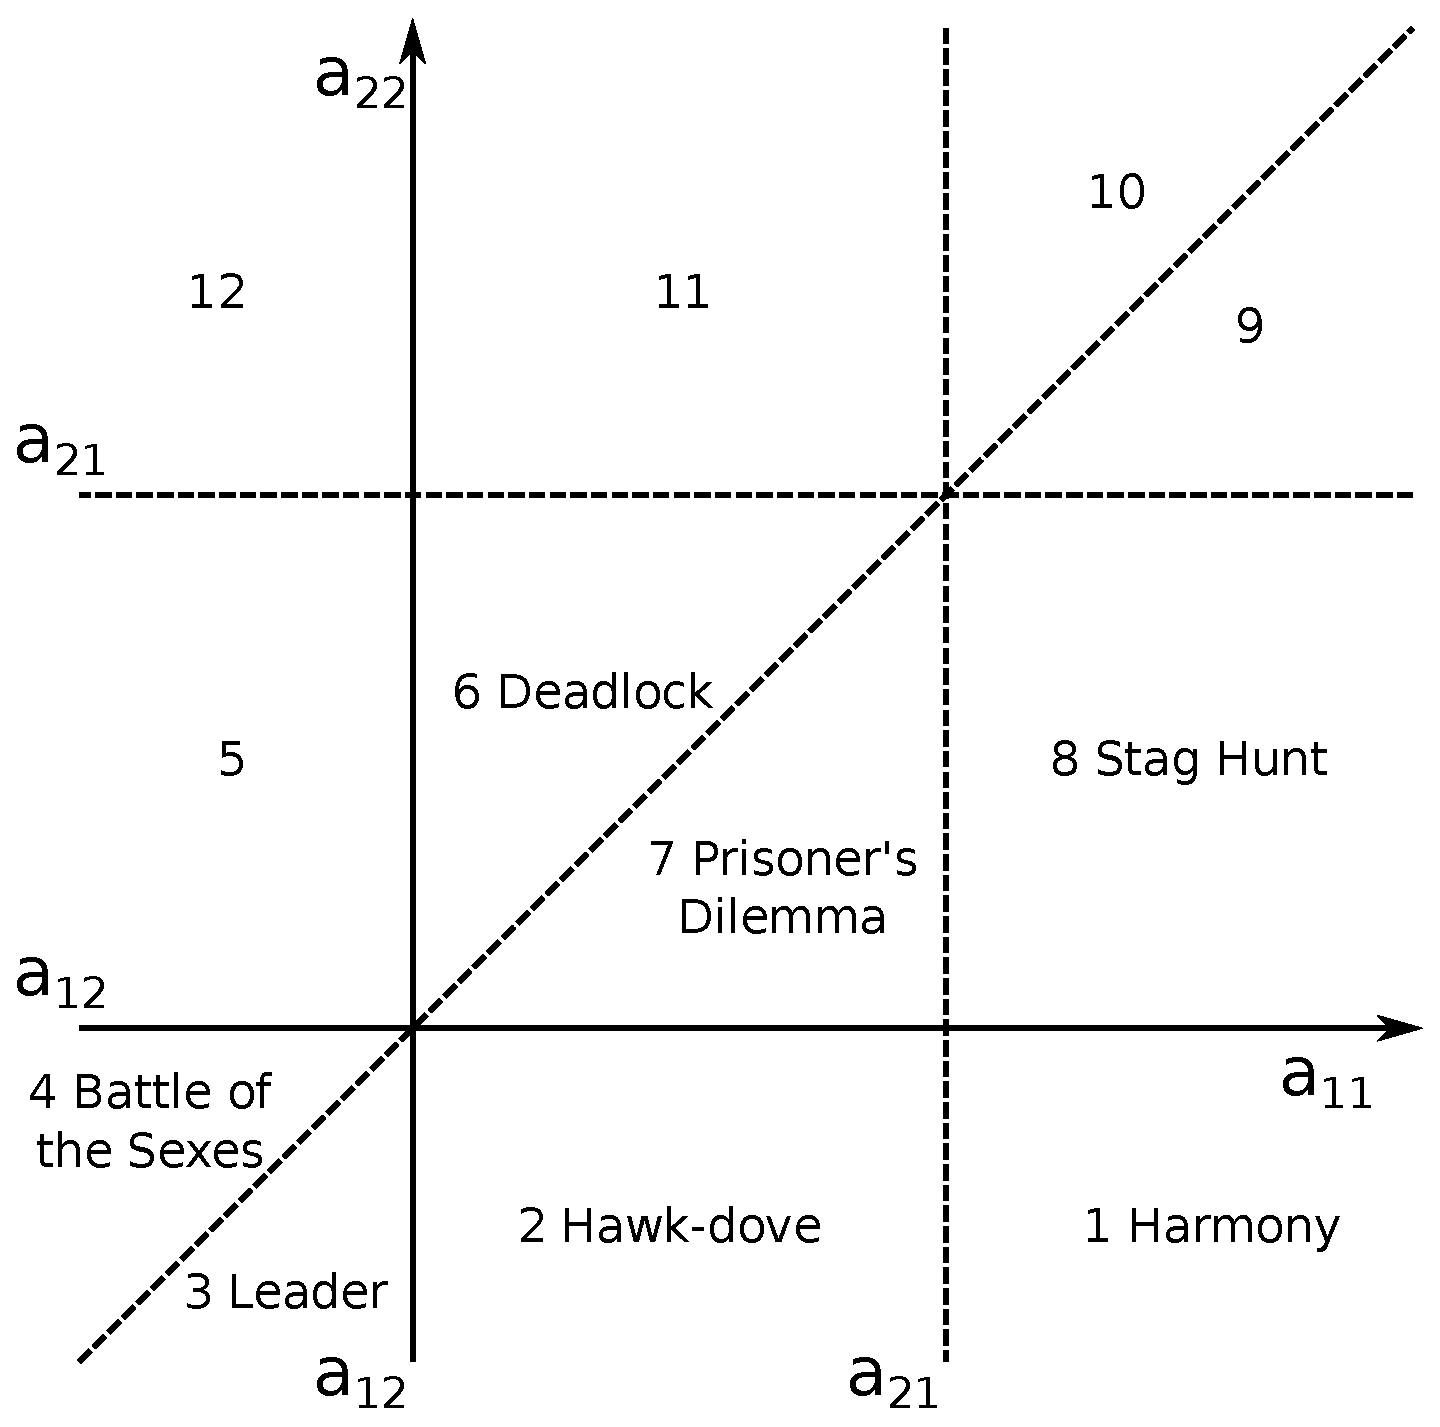
\includegraphics[width=.7\textwidth]{./images/types_of_games_plot.eps}
\caption{
A plot that splits the $a_{11},a_{21}$-plane into twelve regions
based on the orders of payoff coefficients. Each region represents one
class of game.
}
\label{fig:gametypesdiagram}
\end{figure}

\section{A Model With Space and Stochasticity}
\subsection{Interacting particle systems and the voter model}
\label{sec:votermodel}
Our model comes from a partnership between evolutionary game theory
principles and concepts taken from interacting particle
theory. We take a population of players with unchanging
strategies, as in EGT, but rather than allowing them to interact
uniformly at random, we place players on a lattice, one to a site, and
allow interactions to take place only between players in the same
neighborhood. The lattice construction comes from the study of
interacting particle systems, the most basic of which is the voter model.

In the voter model, players' strategies are taken to be opinions on
some topic. Players look to update their strategies at independent,
exponentially distributed times, which, as will be proven later for
a general process of this form, means
that the voter model can be constructed from a collection of Poisson processes. When a player looks to
update her strategy, she chooses one neighbor on the lattice uniformly
at random and adopts the neighbor's strategy. This simple model has
interesting implications in predator-prey models and other situations.

\subsection{Definitions of the processes}
\label{sec:definitions}
We are concerned with seven specific evolutionary game theory
processes, each of which evolves on a lattice. The basic structure of all seven is the same. Take a population of infinitely
many players and arrange them on a
$d$-dimensional lattice. Allow the players to each employ one of $n$
strategies from the set $S = \{1,\dots,n\}$. Let $\eta_t:\mathbb{Z}^d
\to S$ be a function that gives the state of the process at time $t$. Then
$\eta_t(x)$ is the strategy of the player at site $x$ at time $t$. Let
$\sim$ be a relation on $\mathbb{Z}^d$ such that $y\sim x$ if and only
if $y$ is one of the nearest neighbors of $x$ (one unit away from $x$
along any of the $d$ dimensions). Define a function
$N_i:\mathbb{Z}^d\times \mathbb{R}^+\to \mathbb{Z}^+$ such that
$N_i(x,t) = |\{y\sim x:\eta_t(y) = i\}|$, where $|A|$ indicates the
cardinality of the set $A$. Thus, $N_i(x,t)$ denotes the number of
players in the neighborhood of $x$ using strategy $i$ at time $t$. We
also define an $n$-by-$n$ payoff matrix $P$ as

\[
    P = 
    \begin{pmatrix}
      a_{11} & a_{12} & \cdots & a_{1n} \\
      a_{21} & & & \\
      \vdots & & \ddots & \\
      a_{n1} & & & a_{nn}
    \end{pmatrix}.
\]

Define a fitness function
$\phi:\mathbb{Z}^d\times S^{\mathbb{Z}^d} \to \mathbb{R}$ such that
$\phi(x,\eta_t) = \sum_{i=1}^n N_i(x,t)a_{\eta_t(x)i}$. Thus,
$\phi(x,\eta_t)$ denotes the total payoff due to $x$ from all of its
neighbors. With all of this in hand, we can define each of the seven processes rigorously.

\begin{enumerate}[(1)]
\item \emph{Payoff affecting birth and death}

\begin{enumerate}[(a)]
\item \label{itm:1} The player at each site $x$ gives birth at rate $\phi(x,\eta_t)$ if
$\phi(x,\eta_t) > 0$ and dies at rate $-\phi(x,\eta_t)$ if $\phi(x,\eta_t) <
0$. Let $y$ be a site chosen uniformly at random from $\{y':y'\sim
x\}$. When the player at $x$ gives birth, $\eta_t(y) :=
\eta_t(x)$. When the player $x$ dies, $\eta_t(x) := \eta_t(y)$. It is
worth noting that, with payoff matrix
\[
    P = \begin{pmatrix}
      1 & 1 \\
      1 & 1
\end{pmatrix},
\]
this process is identical to the voter model as described in section \ref{sec:votermodel}.

\item \label{itm:2} \emph{Special case: Birth-death updating}

$P$ is restricted such that $a_{ij} \geq 0$ $\forall i,j\in S$. The player at each site $x$ gives birth at rate $\phi(x,\eta_t)$. Let $y$ be a site chosen uniformly at random from $\{y':y'\sim x\}$. When the player at $x$ gives birth, $\eta_t(x) := \eta_t(y)$.
\end{enumerate}

\item \label{itm:3} \emph{Death-birth process}

The player at each site $x$ dies at rate 1 and $\eta_t(x) := i$ with probability
\[
    \frac{\displaystyle\sum_{y\sim x} \phi(y,\eta_t)\mathbbm{1}\{\eta_t(y) = i\}}{\displaystyle\sum_{y\sim x}\phi(y,\eta_t)},
\]
where $\mathbbm{1}$ is equal to 1 when its argument is true and 0 otherwise.

\item \label{itm:4} \emph{Imitation process}

The player at each site $x$ dies at rate 1 and $\eta_t(x) := i$ with probability
\[
    \frac{\displaystyle\sum_{y\sim x} \phi(y,\eta_t)\mathbbm{1}\{\eta_t(y) = i\} + \phi(x,\eta_t)\mathbbm{1}\{\eta_t(x)=i\}}{\displaystyle\sum_{y\sim x}\phi(y,\eta_t) + \phi(x,\eta_t)},
\]
where $\mathbbm{1}$ is equal to 1 when its argument is true and 0
otherwise.

\item \label{itm:5} \emph{Birth-death of the least fit}

The player at each site $x$ gives birth at rate 1. When this occurs,
$\eta_t(y) := \eta_t(x)$, where $y$ is a site chosen uniformly at
random from 
\[
    \left\{ y'\sim x:\phi(y',\eta_t) = \min_{z\sim x}\{\phi(z,\eta_t)\}
    \right\}.
\]

\item \label{itm:6} \emph{Death-birth of the fittest}

The player at site $x$ dies at rate 1. When this occurs, $\eta_t(x) :=
\eta_t(y)$, where $y$ is a site chosen uniformly at random from
\[
    \left\{ y'\sim x:\phi(y',\eta_t) = \max_{z\sim x}\{\phi(z,\eta_t)\}
\right\}.
\]

\item \label{itm:7} \emph{Imitation of the fittest}

The player at site $x$ updates its strategy at rate 1. When this
occurs, $\eta_t(x) := \eta_t(y)$, where $y$ is a site chosen uniformly
at random from \[
    \left\{ y'\sim x \text{ or } y'=x:\phi(y',\eta_t) = \max_{z\sim x\cup
        z=x}\{\phi(z,\eta_t)\} \right\}.
\]

\item \label{itm:8} \emph{Best response dynamics}

The player at site $x$ updates its strategy at rate 1. When this
occurs, $\eta_t(x) := i$, where $i$ is a strategy chosen uniformly at random from 
\[
    \displaystyle\left\{ i':\phi(x,\eta_t | \eta_t(x) = i') = \max_{j\in S}\{\phi(x,\eta_t | \eta_t(x) = j)\} \right\}.
\]
\end{enumerate}

Processes \ref{itm:2}, \ref{itm:3}, and \ref{itm:4} are due to
Ohtsuki et al \cite{ohtsuki}.

\subsection{A mean-field model}
\label{sec:mfm}
The most common way to analyze EGT models is using an ODE derived from
a mean-field approximation in which space is not considered. First, we
classify the seven models into three groups, the members of each of
which behave similarly. Group 1 is process \ref{itm:1} and its special
case, \ref{itm:2}. Group 2 is processes \ref{itm:3} and \ref{itm:4},
and we call these linear processes, since a new strategy is chosen
with probability linearly proportional to its fitness. Group 3 is
processes \ref{itm:5}, \ref{itm:6}, and \ref{itm:7}, and
we call these nonlinear processes, since a new strategy is chosen with
a probability either 1 or 0, depending on its fitness. Process
\ref{itm:8} stands alone, because its behavior is in some ways quite
different from the behaviors of the other processes.

We will first present a mean-field model (MFM) for the first group. Both of the processes give the
same MFM, because the latter is simply a special case of the former in
which only positive payoff is considered. First, we need
some definitions. Let $X_i$ be the proportion of strategy $i$ in the population. Thus, $X_1+X_2 = 1$ at all times $t$. In the context of
MFM's, we define the fitness function $\phi_i(\vec{X}) = \phi_i(X_1,X_2)$
as the fitness of type $i$. Then $\phi_i(\vec{X}) =
\sum_{j=1}^n a_{ij}X_j$, where $n$ is the number of
strategies. For our purposes, $n=2$, so $\phi_i(\vec{X}) = a_{i1}X_1 +
a_{i2}X_2$.

We construct the MFM for payoff affecting birth and
death around $\frac{d X_1}{dt}$, which uniquely determines $\frac{d
  X_2}{dt}$, since $X_1+X_2=1$ at all times. $X_1$ changes in one of
two ways. In the first, a site $x$ of strategy 1 is chosen, which
occurs with probability $X_1$. The player at $x$ must then give birth or die, which occurs at rate
$|\phi_1(\vec{X})|$ and affects $X_1$ according to its sign.
Finally, a site of strategy 2 must be chosen to replace (if the player at
$x$ died) or be replaced (if the player at $x$ gave birth), which
occurs with probability $X_2$. Thus, the first term in the MFM is the
product of these three probabilities, $X_1\phi_1(\vec{X})X_2$. The other way for $X_1$ to change is exactly symmetrical, but with
strategy 2 chosen to begin with and strategy 1 chosen to replace or be
replaced. This second way has the opposite effect on $X_1$, so this
term has the opposite sign. Therefore,
\begin{align*}
    \frac{dX_1}{dt} &= X_1\phi_1(\vec{X})X_2 - X_2\phi_2(\vec{X})X_1
    \\
    &= X_1X_2\left(\phi_1(\vec{X})-\phi_2(\vec{X})\right).
\end{align*}

This differential equation is known as the replicator equation, and it
is used throughout EGT to describe many phenomena. 

We can analyze this ODE with a bifurcation diagram. To construct a
bifurcation diagram, we fix $a_{21}$ and $a_{12}$ and allow $a_{11}$
to vary along the $x$-axis and $a_{22}$ to vary along the
$y$-axis, centering the diagram at the point $(a_{21},a_{12})$. We must analyze
the differential equation's asymptotic behavior in each quadrant of
this diagram. Let $a_1 = a_{11}-a_{21}$ and $a_2 = a_{22}-a_{12}$, so
that the two axes of the diagram are equivalent to $a_1$ and $a_2$. Recalling that
$X_2 = 1-X_1$, we can write the replicator equation as

\begin{align*}
    \frac{dX_1}{dt} &= X_1(1-X_1)\left(a_1X_1 - a_2(1-X_1)\right) \\
    &= X_1(1-X_1)\left( (a_1+a_2)X_1 - a_2 \right).
\end{align*}

There are clearly three fixed points at $X_1=0$, $X_1=1$, and
$X_1=\frac{a_2}{a_1+a_2}$. We investigate equilibrium behavior of the
equation in between the fixed points in each of the four regions of the bifurcation diagram.

\begin{enumerate}[I.]
\item $a_1, a_2 > 0$.

If $1 > X_1 > \frac{a_2}{a_1+a_2}$, then $(a_1+a_2)X_1 - a_2 > 0$, so
  $\frac{dX_1}{dt} > 0$. If $0 < X_1 < \frac{a_2}{a_1+a_2}$, then $(a_1+a_2)X_1 - a_2 < 0$, so
  $\frac{dX_1}{dt} < 0$. So, on
  either side of the fixed point, $X_1$ is pushed towards one edge or
  the other, but which strategy wins is determined only by the
  initial conditions. Therefore, we have a bistable equilibrium in
  this quadrant.

\item $a_1<0$, $a_2>0$.

  In this case, we should consider the form
\[
    \frac{dX_1}{dt} = X_1(1-X_1)(a_1X_1 - a_2X_2).
\]
Clearly, $\frac{dX_1}{dt} < 0$ for all values of $X_1$, as $X_1>0$ and
$1-X_1>0$, but $a_1X_1 < 0$ and $a_2(1-X_1) > 0$. This means that at
equilibrium strategy 2 will dominate the lattice.

\item $a_1,a_2<0$.

  Here, we have a mirror image of the case in quadrant I. If $1 > X_1 > \frac{a_2}{a_1+a_2}$, then $(a_1+a_2)X_1 - a_2 < 0$, so
  $\frac{dX_1}{dt} < 0$. If $0 < X_1 < \frac{a_2}{a_1+a_2}$, then $(a_1+a_2)X_1 - a_2 > 0$, so
  $\frac{dX_1}{dt} > 0$. So, on either side of the fixed point, $X_1$ is forced
  back towards the fixed point. Therefore, we have a coexistent
  equilibrium in this quadrant.

\item $a_1>0$, $a_2<0$.

  Here, we have a mirror image of the case in quadrant
  II. $\frac{dX_1}{dt} > 0$ for all values of $X_1$, as all factors on
  the right hand side are necessarily positive. This means that at equilibrium strategy 1 will dominate the lattice.

\end{enumerate}

\begin{figure}[h]
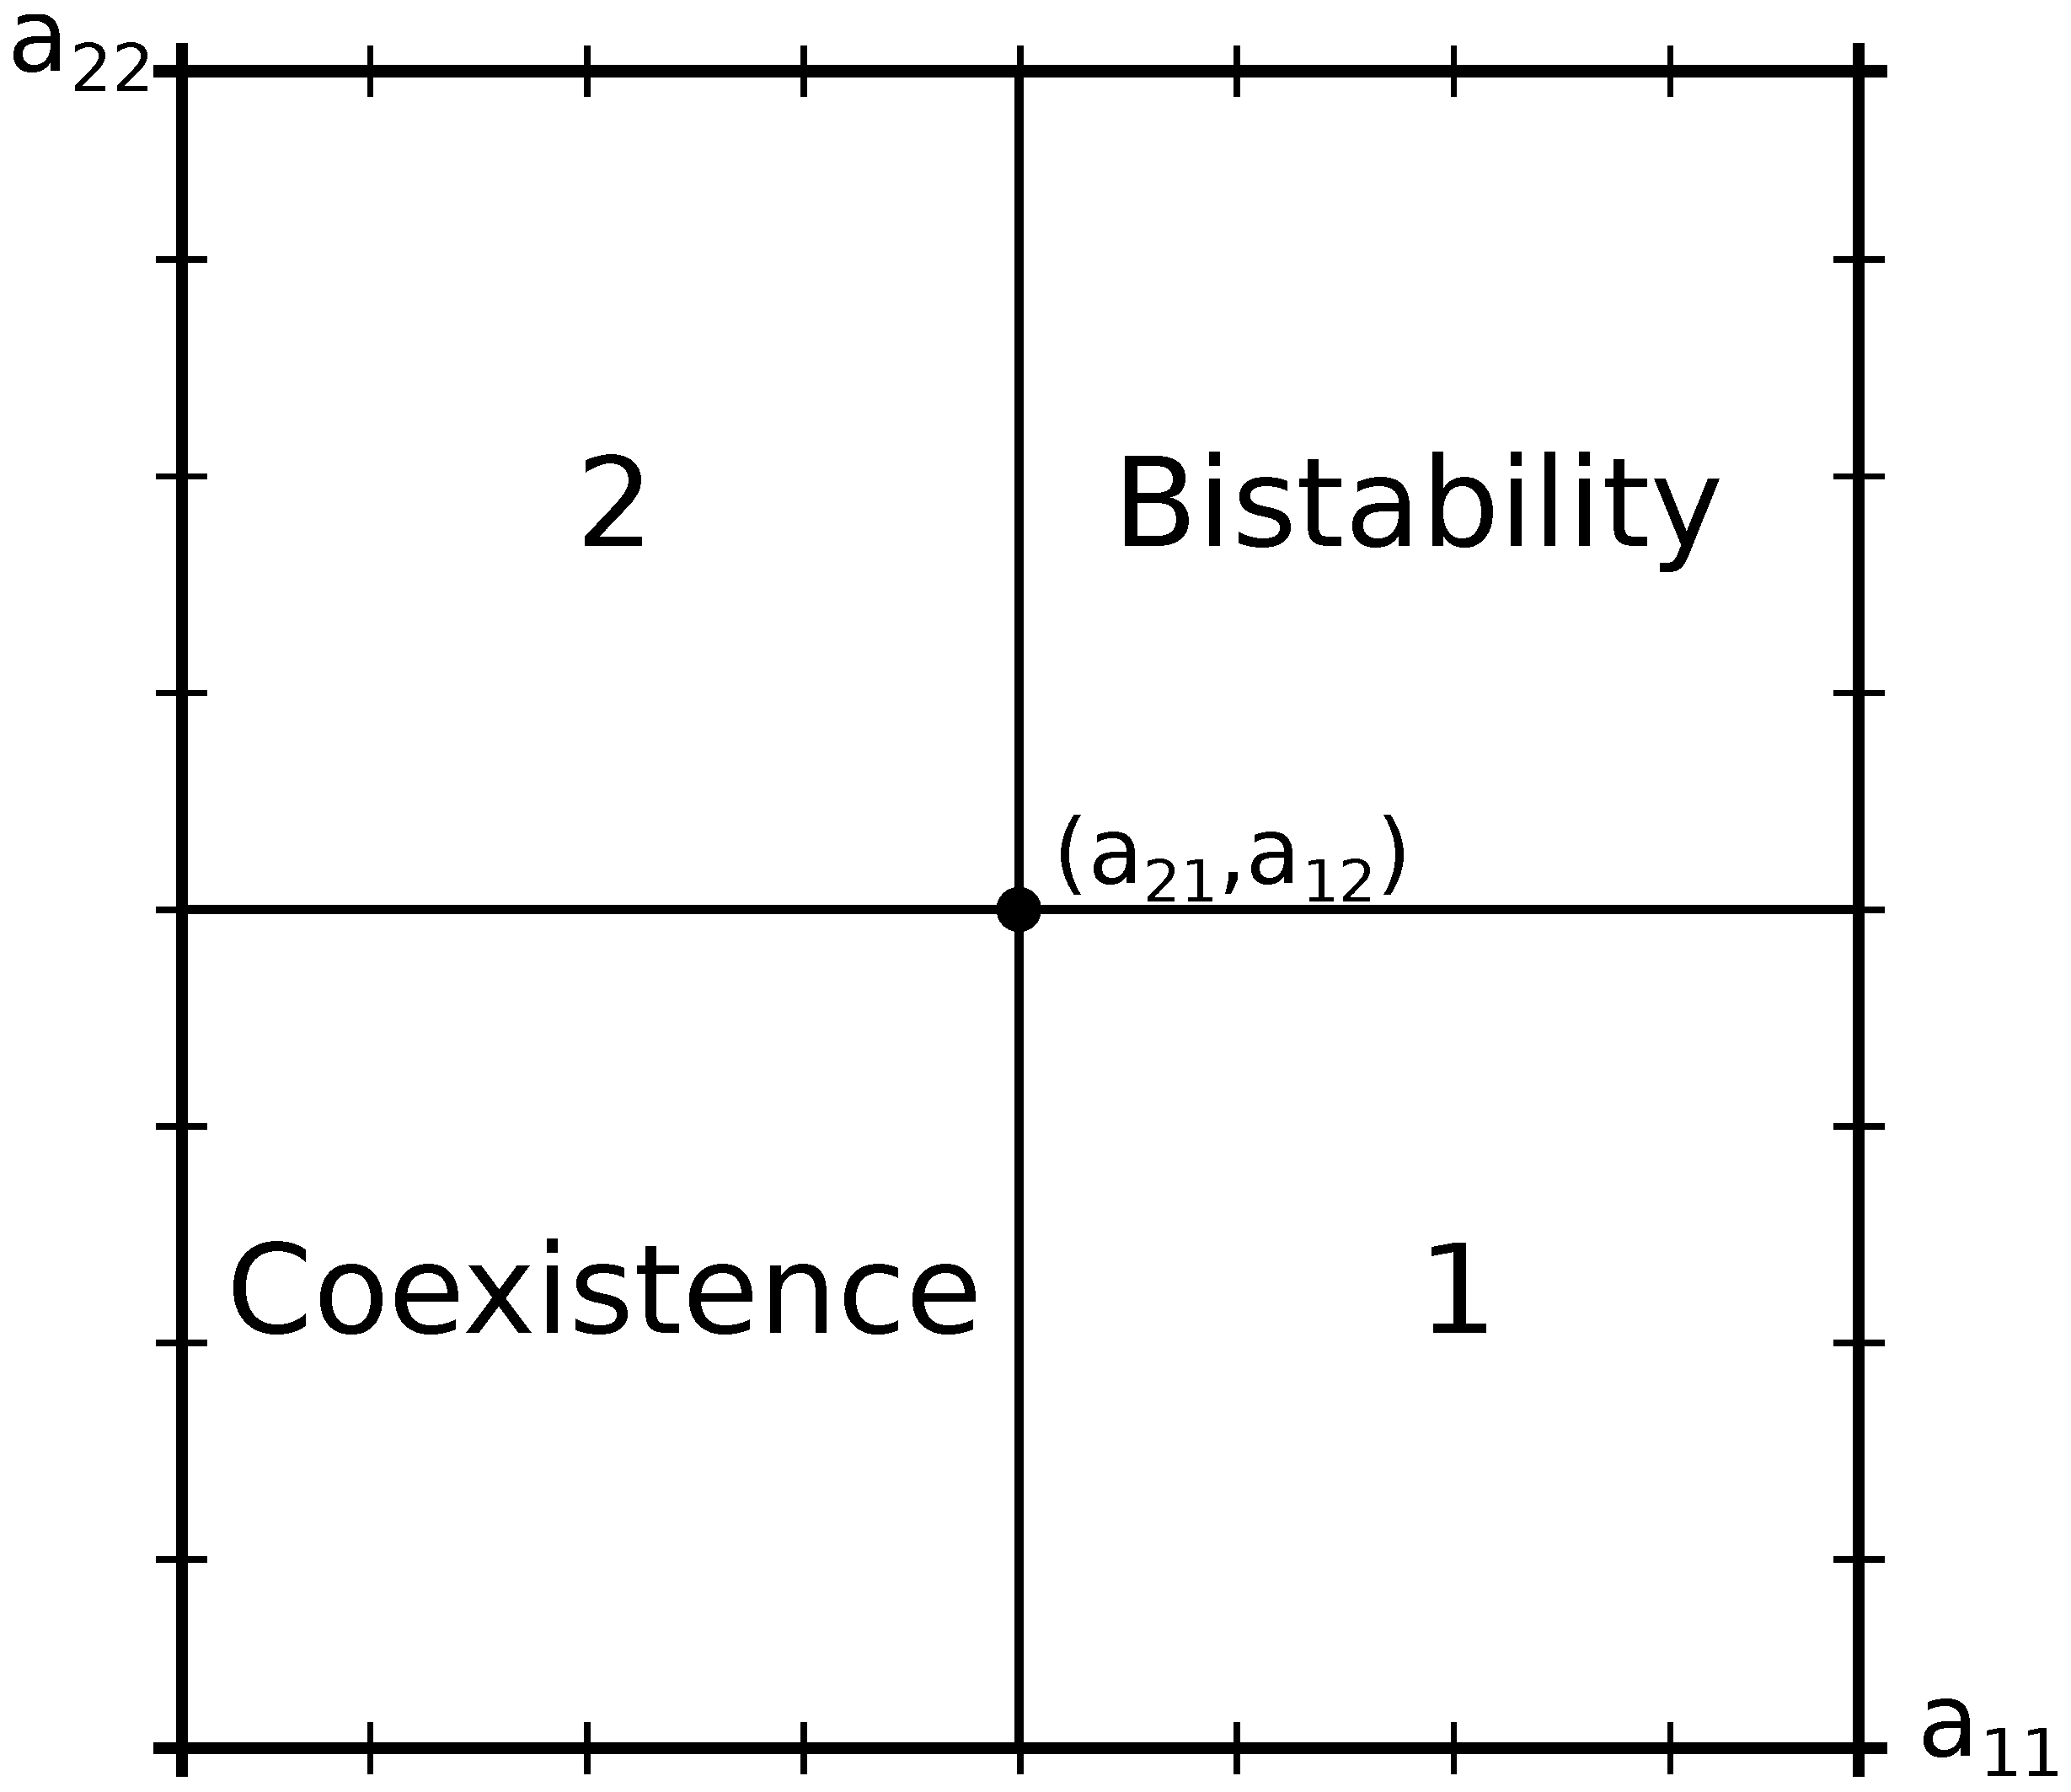
\includegraphics[width=.5\textwidth]{./images/replicator_bifurcation_diagram.eps}
\caption{The bifurcation diagram for the replicator equation, showing
  the long-term behavior of our EGT processes for varying payoff
  matrices. The fixed point at the center is the point at which
  $a_{11} = a_{12}$ and $a_{22} = a_{21}$.}
\label{fig:replicatorbifurcationdiagram}
\end{figure}

Figure \ref{fig:replicatorbifurcationdiagram} simply shows what we
observed above: in each quadrant, we have a different kind of
long-term behavior. We will see immediately that the other two classes
of processes exhibit similar behavior in the long run. Later on, we will
see that the spatially dependent versions of these processes show some
kinds of comparable behaviors.

We now construct MFM's for group 2 processes, which differ only in
the definition of the neighborhood of $x$ as including $x$ or
not. Clearly, these are the same in a well-mixing population, since
all sites are neighbors of each other regardless of this spatial condition.

This MFM is also constructed around $\frac{d X_1}{dt}$. $X_1$ can
again change in two ways. In the first, a player of strategy 2
must be selected to die, which occurs with probability
$X_2$. A player of strategy 1 must be selected to replace it,
which occurs with probability equal to the proportional payoff of
strategy 1, $\frac{X_1\phi_1(\vec{X})}{X_1\phi_1(\vec{X}) +
  X_2\phi_2(\vec{X})}$. As before, the second way $X_1$ can change is
symmetric and of the opposite sign, so we have the differential
equation
\begin{align*}
  \frac{d X_1}{dt} &= X_2 \frac{X_1\phi_1(\vec{X})}{X_1\phi_1(\vec{X}) +
  X_2\phi_2(\vec{X})} - X_1 \frac{X_2\phi_2(\vec{X})}{X_1\phi_1(\vec{X}) +
  X_2\phi_2(\vec{X})} \\
  &= \frac{X_1 X_2 \left( \phi_1(\vec{X}) -
      \phi_2(\vec{X})\right)}{X_1\phi_1(\vec{X}) + X_2\phi_2(\vec{X})}.
\end{align*}

Notice that this equation is quite similar to the replicator equation,
and, in fact, the analysis of the two equations is the same. If we
were to construct a bifurcation diagram as before, we would see an
identical picture.

The final MFM is for the group 3 processes. We again construct the model around $\frac{d X_1}{dt}$,
and, again, $X_1$ can change in one of two ways. In the first, a site
of strategy 2 is selected to update, which happens with probability
$X_2$. All that remains is for $\phi_1(\vec{X})-\phi_2(\vec{X}) > 0$,
that is, for strategy 1 to be the best response for the chosen
site. We identify this using the indicator function
$\mathbbm{1}\{\phi_1(\vec{X})-\phi_2(\vec{X}) > 0\}$, which is 1 when
its argument is true and 0 otherwise. The second way that $X_1$ can
change is again symmetric and oppositely signed, so the MFM is

\begin{align*}
    \frac{d X_1}{dt} &=
    X_2\mathbbm{1}\{\phi_1(\vec{X})-\phi_2(\vec{X}) > 0\} -
    X_1\mathbbm{1}\{\phi_1(\vec{X})-\phi_2(\vec{X}) < 0\}.
\end{align*}

Though this equation appears quite different from the first two
models, analysis again shows that the limiting behavior of the
process is similar; all that changes is how fast the process will
converge to the fixed points depending on the payoff matrix. Again, the bifurcation diagram is identical.

\subsection{Justification of a Poisson process on an infinite lattice}

We now address a concern that may arise with use of the infinite
lattice. Because there are infinitely many sites and therefore
infinitely many players, we may have trouble defining which site is
the first to update. In more concrete terms, we have $\min\{X\}$,
where $X$ is a set of infinitely many exponential random variables. In
general, the minimum of a countably infinite set of exponential random
variables is not defined. In order to prove that the minimum is in
fact defined on the infinite lattice, we must use an argument of
Harris by way of Durrett \cite{harris}\cite{durrett}.

Let $t_0 > 0$ be small. We say that sites $x$ and $y$ are connected if
$x$ has been selected for update by time $t_0$ and the payoff of $y$
was considered in deciding how $x$ should update (thus, $y\sim
x$). This divides the lattice into connected components based on
selection of the time $t_0$. Clearly, each of these connected
components must be entirely independent of the others, since no
communication of any kind has taken place between
components. All that is left is to show that

\begin{thm}
  If $t_0$ is sufficiently small, then all connected components of the
  lattice are finite with probability 1.
\end{thm}

With that result, which is left unproven here, we can determine a
first selected site in each component. In turn, we can establish the
evolution of the process from time 0 to time $t_0$. Following
this, we can establish the evolution from time $t_0$ to a similarly
small time $t_1 > 0$, and so on \textit{ad infinitum}.

\section{Simulation and Justification}

\subsection{Simulation of the processes}

We are obviously unable to simulate these process exactly, as an
infinite lattice cannot be stored in finite memory. To combat this, we
instantiate a finite lattice as an array of integers and give it periodic boundary
conditions. This means that, in the interior of the lattice, nearest
neighbors are defined as members above, below, and to either side of
the point in question, but at the edges, the neighborhoods ``wrap around''
the lattice, so that an edge particle interacts with its neighbors
on the edge, one away from the edge, and a fourth site on the
opposite edge. We can visualize this as wrapping a square lattice
around a torus, as seen in Figure \ref{fig:periodictorus}.

\begin{figure}[h t]
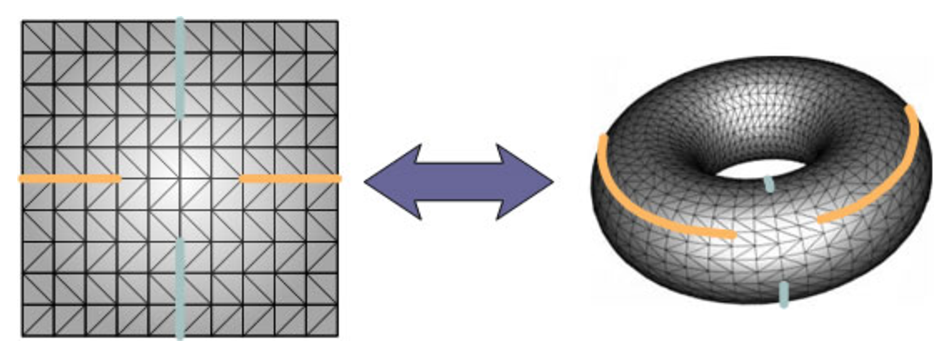
\includegraphics[width=.7\textwidth]{./images/torus.eps}
\caption{A 2D grid wrapped around a torus, representing periodic
  boundary conditions\cite{website:ising-model}.}
\label{fig:periodictorus}
\end{figure}

Once we have built the lattice in code, we must establish a method for
choosing which site will be updated at any given time. In the formal
definitions, we describe this as occurring ``at rate 1'', which means that updates occur at the times of a Poisson process
with rate parameter 1. In order to simulate this, we employ the
Law of Large Numbers, which states that, for any random variable
$X$, $\displaystyle\pr\left(\lim_{n\to\infty} \overline{X_n}=\E(X)\right) = 1$, where $X_n$ is
a vector of $n$ results from the distribution of $X$, and
$\overline{X_n}$ is the average of these results. Because any
interesting simulation of this process will go through tens of
thousands of iterations, $n$ is certainly large, so we can say that
the time between updates will be approximately the expected value:
1. Because the timescale is arbitrary, we allow updates to occur
as often as the computer is capable.

We must also establish a method with which to determine which site
updates when. To do this, we use a well-worn result from probability theory.

\begin{lem}
  If $T_1,\dots, T_n$ is a collection of $n$ independent exponential
  random variables with rate parameters $\lambda_1,\dots, \lambda_n$,
  then $\displaystyle\pr\left( T_i =
  \min\{T_1,\dots, T_n\} \right) = \frac{\lambda_i}{\sum_{j=1}^n\lambda_j}$.
\end{lem}
\label{lem:minofexponentials}

\begin{proof}
\begin{align*}
  \pr(T_i = \min\{T_1,\dots,T_n\}) &= \pr(X_i<X_j \forall j\neq i) \\
  &= \int_0^\infty \pr(X_i<X_j\forall j\neq i | X_i=t) \pr(X_i=t)dt \\
  &= \int_0^\infty \lambda_i e^{-\lambda_i t}\prod_{j\neq i} \pr(X_j >
  t) dt \\
  &= \lambda_i \int_0^\infty e^{-\lambda_i t}\prod_{j\neq i}
  e^{-\lambda_j t} dt \\
  &= \lambda_i \int_0^\infty e^{-(\lambda_1+\dots+\lambda_n)t} dt \\
  &= -\lambda_i \left[
    \frac{e^{-(\lambda_1+\dots+\lambda_n)t}}{\sum_{i=1}^n \lambda_i}
  \right]_0^\infty \\
  &= \frac{\lambda_i}{\lambda_1+\dots+\lambda_n}. \qedhere
\end{align*}
\end{proof}

In our situation, we have $n$ independent and identically distributed
exponential random variables with rate parameter 1, so the probability
that any one site is the next to update is $\frac{1}{n}$. In terms of
simulating, this means that at each update time (i.e., as often as
the computer is able) we select one of the sites uniformly at random.

Now that we have a lattice on which to place players and a method by
which to select them for update, it remains only to discuss what
occurs during an update. The details, of course, vary according to the
definitions of the models as outlined in section
\ref{sec:definitions}. In general, though, payoff is computed for the
selected site and its four nearest neighbors based upon the
strategies of the surrounding neighbors, and then a random number is
generated to determine the new strategy of the node in question. It is
perhaps best to see an example; the Java code in the following code listing details updating under process \ref{itm:1}.

\begin{samepage}
\begin{lstlisting}
public void updateMethodZero2D(Point node)
{
		double payoff = getPayoff2D(node);
		// Negative payoff => death rate. If the node dies, we replace it with a copy of a random neighbor.
		if (payoff < 0)
        {
            if (rand.nextDouble() <= (-payoff / getMaxRate()))
            {
				Point neighbor = chooseNeighborAtRandom2D(node);
				setStrategyAt2D(node, array[neighbor.x][neighbor.y]);
			}
		}
		// Positive payoff => birth rate. If the node gives birth, we replace a random neighbor with a copy of (node).
		else if (payoff > 0)
		{
			if (rand.nextDouble() <= (payoff / getMaxRate()))
			{
				Point neighbor = chooseNeighborAtRandom2D(node);
				setStrategyAt2D(neighbor, array[node.x][node.y]);
			}
		}
	}
\end{lstlisting}
\end{samepage}

We start by getting the payoff of the player at the updating site. As
per the description of the process, if the payoff is negative, the
site ``dies'', and if the payoff is positive it ``gives birth''. In
either case, we generate a random rational number between 0 and 1 and
compare it to the payoff divided by the maximum possible payoff
(given by the function \texttt{getMaxRate()} in the code). This division
normalizes the birth rate so that if maximum payoff is attained by a
selected node, the probability of birth is 1. If the random number test is passed, we choose a random neighbor of the updating site and either (1) copy the neighbor's strategy to the updating site (if the updating site ``dies''), or (2) copy the updating site's strategy to the neighboring site (if the updating site ``gives birth'').

There are comparable methods for the other process, with the end result being real-time, animated simulations of the seven EGT models. The simulation is the source of 

\subsection{The poisson lemma}
In order for our descriptions of the processes to be consistent, we must
prove that the general updating process is in fact Poisson. Let $X_t$ be a Poisson process that counts the number of
points in the Poisson point process with rate parameter $\mu$. Let
$Y = \{Y_i: i\in\mathbb{N}\}$, be a set of independent and identically
distributed Bernoulli random variables with parameter $p$. We will say
that the $i$th point of the Poisson point process is an update point
if $Y_i = 1$. 
Then we can state the following lemma:
\begin{lem}
Let $\overline{X_t}$ be the number of update points of
the Poisson point process in the interval $[0,t]$. Then $\{\overline{X_t} : t\geq
0\}$ is a Poisson process with rate parameter $\mu t p$.
\end{lem}
\begin{proof}
By conditioning on all the possible values of $X_t$, we can easily see that
\[
    \pr(\overline{X_t} = k) = \sum_{j=k}^\infty \pr(\overline{X_t}=k |
    X_t = j)\pr(X_t=j).
\]
$\pr(\overline{X_t}=k|X_t=j)$ is
the probability of finding $k$ update points among $j$ points, which,
by construction, is clearly the probability that a Binomial$(j,p)$
random variable is equal to $k$. Thus,
\[
    \pr(\overline{X_t}=k|X_t=j) = {j\choose k} p^k (1-p)^{j-k}.
\]
Substituting into the above series and using that $X_t\sim Poisson(\mu
t)$, we find
\begin{align*}
    \pr(\overline{X_t} = k) &= \sum_{j=k}^\infty {j\choose k}
    p^k(1-p)^{j-k} \frac{(\mu t)^j}{j!} e^{-\mu t} \\
    &= \frac{e^{-\mu t} p^k}{k!} \sum_{j=k}^\infty \frac{(\mu t)^j
      (1-p)^{j-k}}{(j-k)!} \\
    &= \frac{e^{-\mu t} (\mu t p)^k}{k!} \sum_{j=0}^\infty \frac{(\mu t(1-p))^j}{j!}.
\end{align*}
Notice that the series portion is the Taylor expansion of $e^{\mu t
  (1-p)}$. Therefore, we have
\begin{align*}
    \pr(\overline{X_t}=k) &= \frac{(\mu t p)^k}{k!} e^{-\mu t}e^{\mu t
      (1-p)} \\
    &= \frac{(\mu t p)^k}{k!} e^{-\mu t p}.
\end{align*}
Thus, $\overline{X_t} \sim \text{Poisson}(\mu p t)$. In turn, this
implies that $\{\overline{X_t} : t\geq 0\}$ is a Poisson process with
intensity $\mu p$.
\end{proof}

\section{Results}

\subsection{Domination, coexistence, and clustering}
In any of these processes,
there are three distinct types of long-term behaviors: (1) one strategy dominates
the lattice; (2) strategies cluster, each dominating some subset of
the lattice but with no strategy controlling the whole lattice;
(3) strategies coexist, meaning that no strategy takes control even of an
appreciable proportion of the lattice. The rigorous definition of domination is obvious: the proportion of the dominating strategy becomes equal to 1. We say that clustering occurs when
\[
    \lim_{t\to\infty} \pr\left(\eta_t(x) \neq \eta_t(y)\right) = 0,\; \forall x,y\in\mathbb{Z}^d,
\]
that is, when the asymptotic probability that any pair of sites will have different strategies is zero. Coexistence occurs when
\[
    \lim_{t\to\infty} \pr\left(\eta_t(x)\neq\eta_t(y)\right) > 0,\; \forall x,y\in\mathbb{Z}^d,
\]
that is, when the aforementioned probability is non-zero. These descriptions will be instrumental in describing the simulated behavior of the processes.

\subsection{Bifurcation diagrams}
The best way to see the impact of space and stochasticity on these
processes is to overlay the spatial bifurcation diagrams on the MFM
diagram from section \ref{sec:mfm}. The forthcoming diagrams were
created from examination of simulations, so it is necessary to choose
the fixed point, $(a_{21},a_{12})$, which we have set to $(3,6)$. As
the remaining two parameters vary, we see behaviors that are
comparable to those predicted by the mean-field model.

\begin{figure}[h]
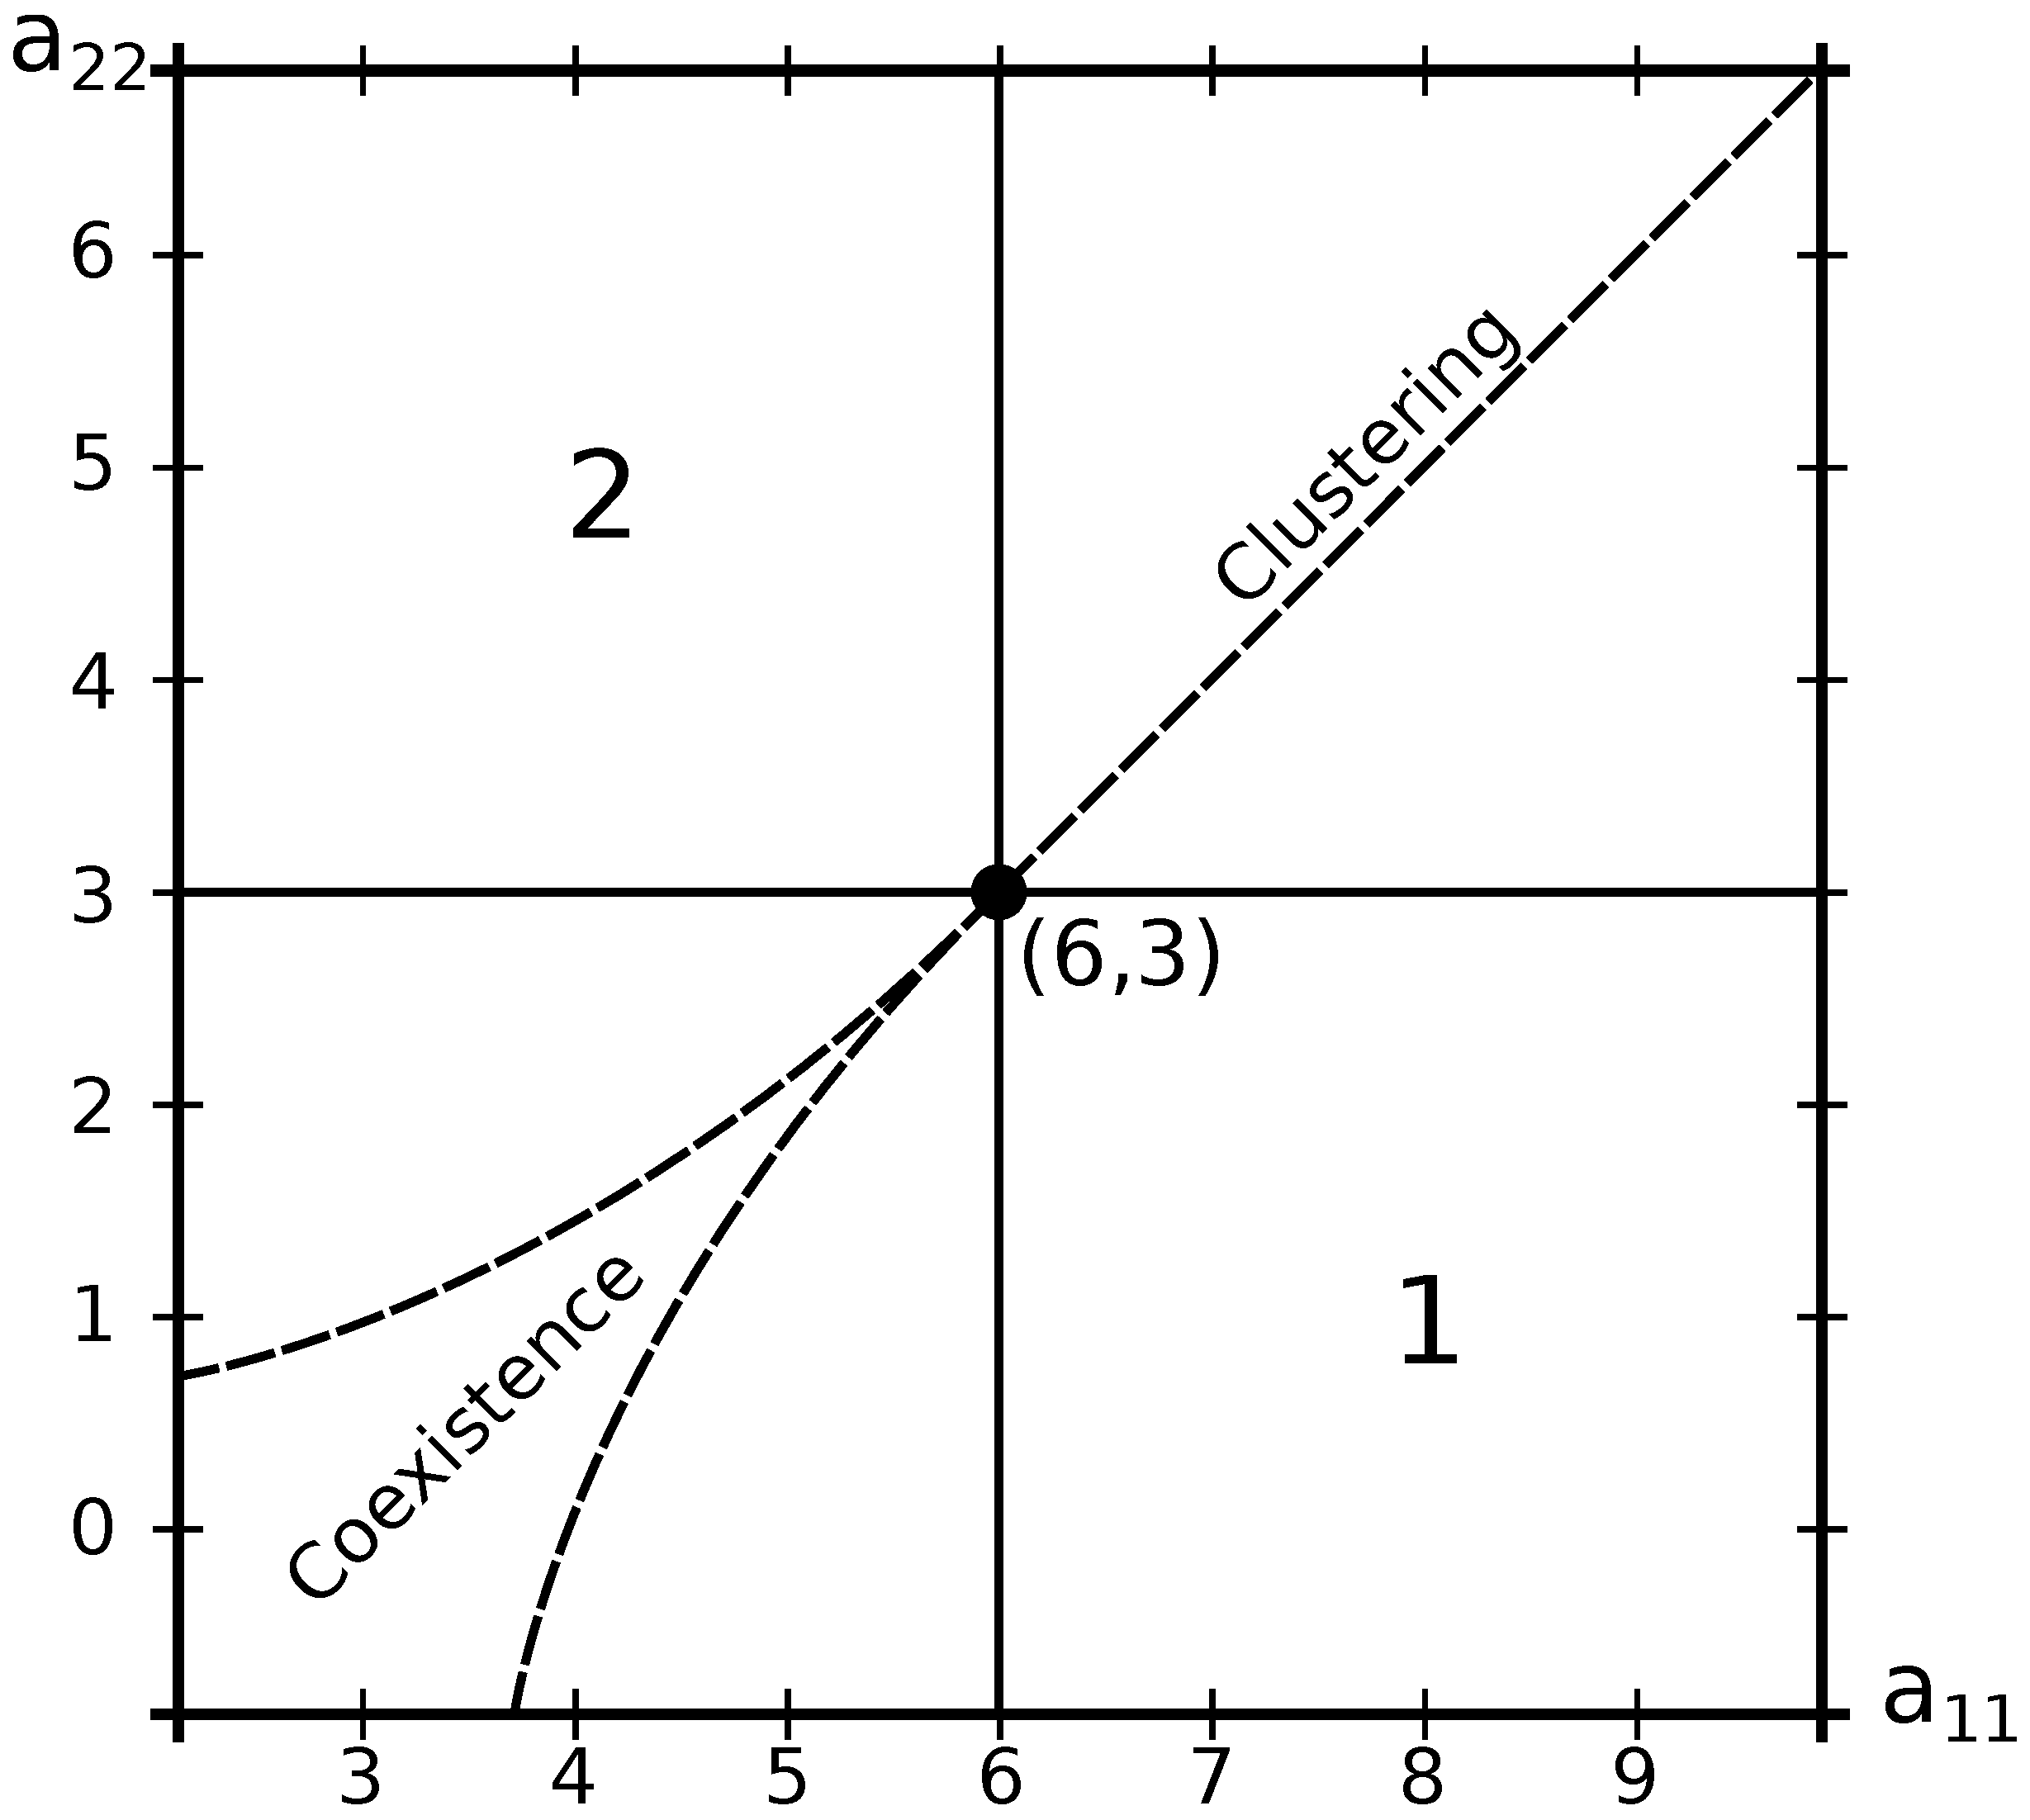
\includegraphics[width=0.5\textwidth]{./images/group_1_bifurcation_diagram.eps}
\caption{
A bifurcation diagram for process \ref{itm:1}. The behavior of process \ref{itm:2} is analogous. These results are extrapolated from multiple long-run simulations.
}
\label{fig:group1diagram}
\end{figure}

In Figure \ref{fig:group1diagram}, we can see similarities to the
bifurcation diagram for the mean-field model in section \ref{sec:mfm},
but there are two key differences. First, in quadrant I, one strategy or the
other dominates the lattice in most situations, but in configurations
along the dotted line, we see clustering behavior. Also, in quadrant
III, we again see domination in most situations, but configurations in
the region between the two dotted curves result in coexistence
behavior.

\begin{figure}[h]
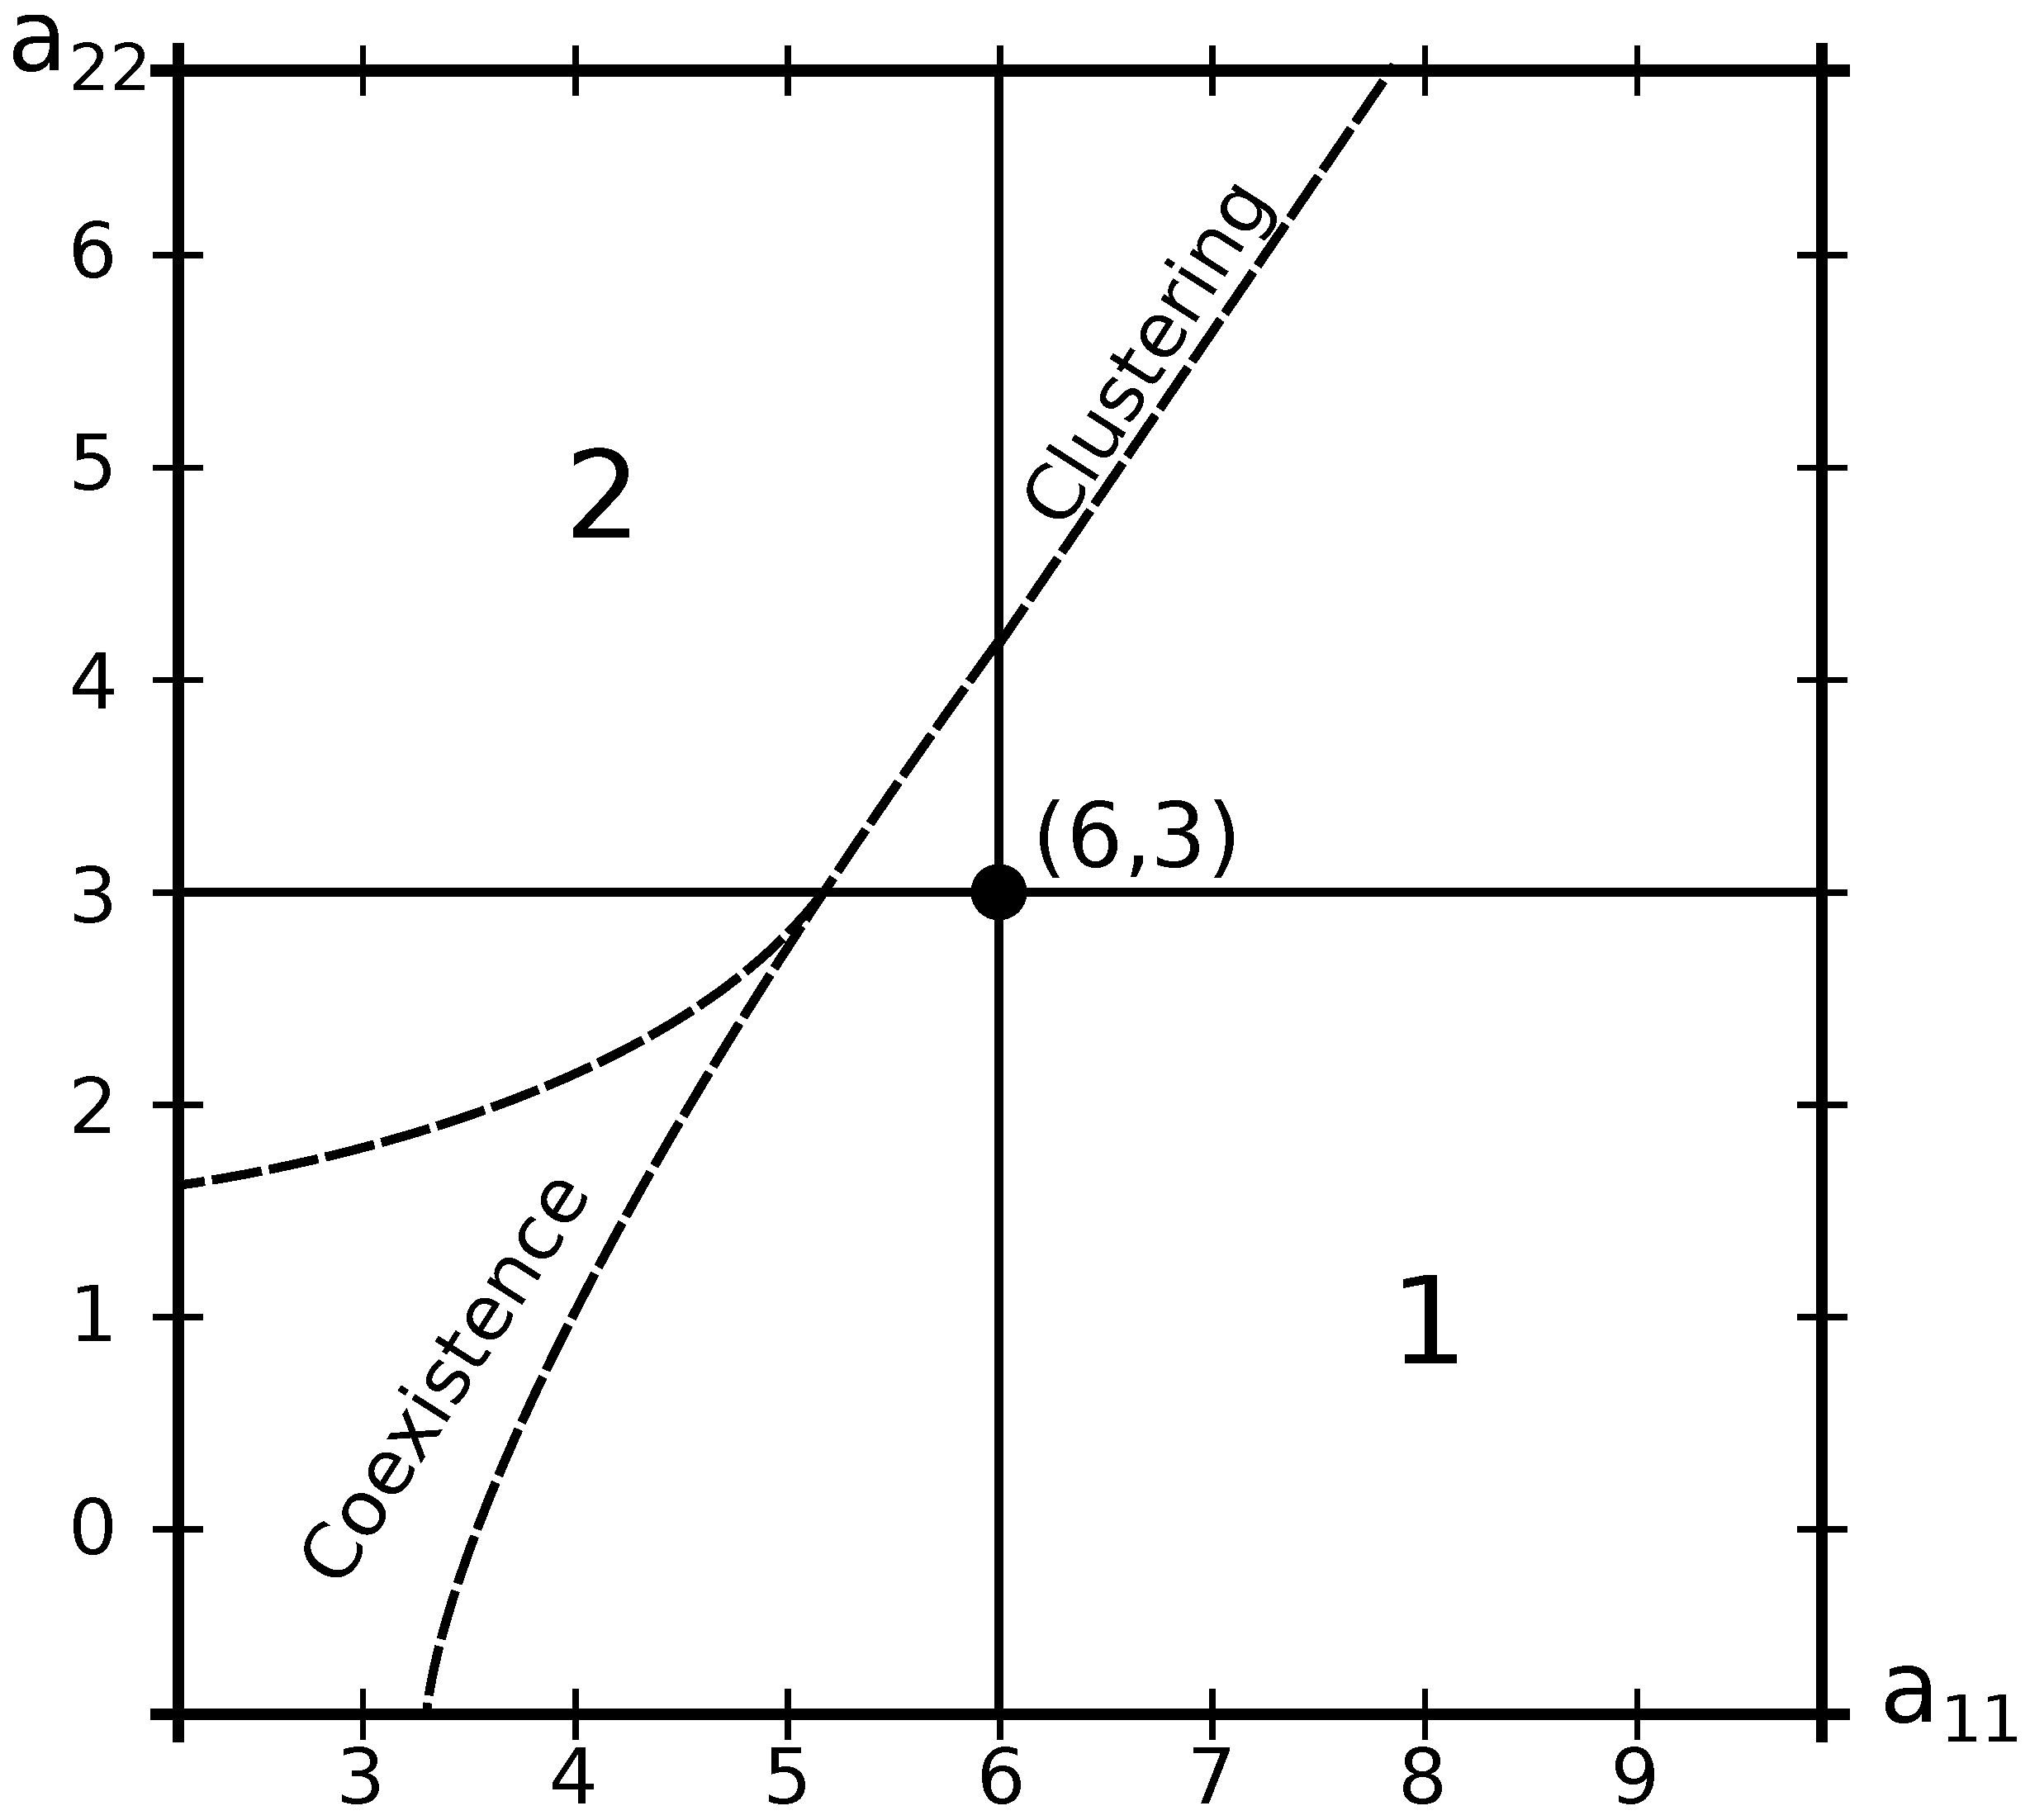
\includegraphics[width=0.5\textwidth]{./images/group_2_bifurcation_diagram.eps}
\caption{
A bifurcation diagram for process \ref{itm:3}. The behaviors of
processes \ref{itm:3} and \ref{itm:4} are analogous.
}
\label{fig:group2diagram}
\end{figure}

Figure \ref{fig:group2diagram}, which shows behavior of group 2
processes, reveals similar behaviors to those in Figure
\ref{fig:group1diagram}. However, we see that the clustering line in
quadrant I is shifted up and to the left of the fixed point
$(6,3)$. In quadrant III, we still see a region of coexistence as the
clustering line splits, but the region is skewed to the left of what
it was for group 1 processes.

\begin{figure}[h]
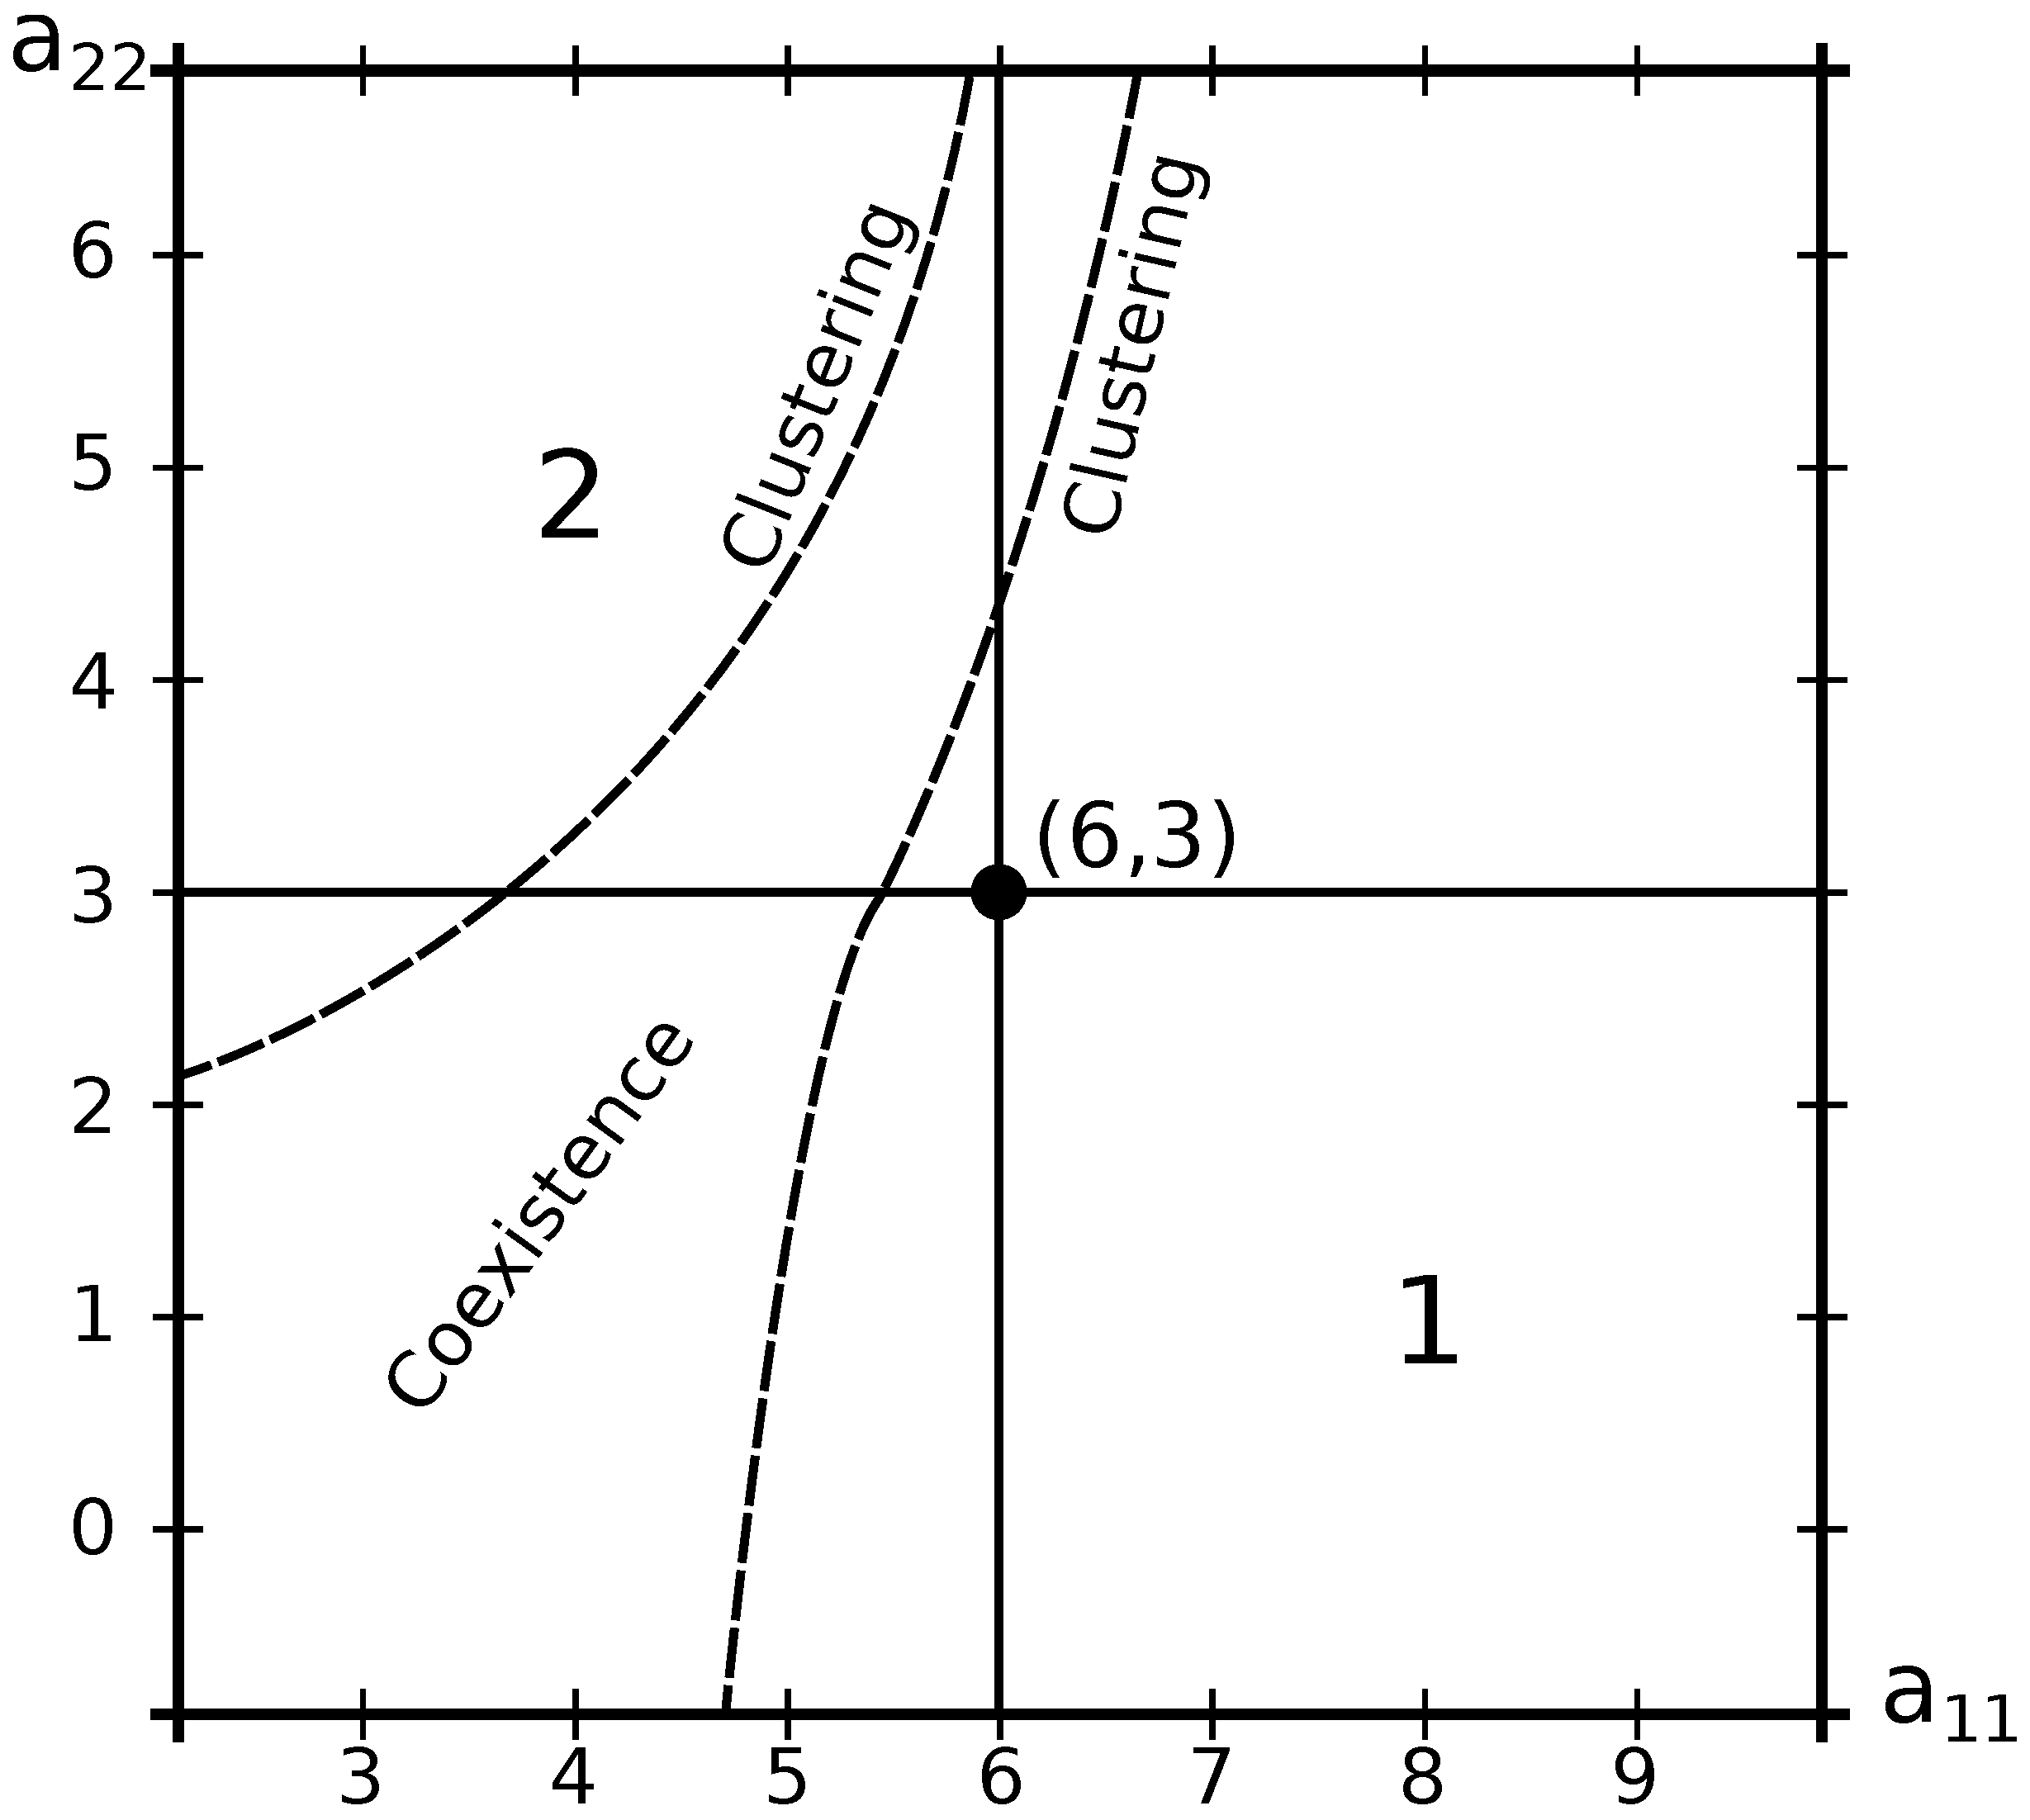
\includegraphics[width=0.5\textwidth]{./images/group_3_bifurcation_diagram.eps}
\caption{
A bifurcation diagram for process \ref{itm:6}. The behaviors of
processes \ref{itm:5} and \ref{itm:7} are analogous.
}
\label{fig:group3diagram}
\end{figure}

Figure \ref{fig:group3diagram} shows a departure from the behaviors of
groups 1 and 2, as clustering regions are along two distinct lines,
rather than one that splits upon crossing the x-axis. Moreover,
clustering behavior is quite different for this process. Because the
update process is based upon the highest-payoff neighbor, the behavior
tends to be more deterministic than the ``linear'' models in which
the probability of a switch correlates directly with the payoffs of
surrounding strategies. As a result, long-term behavior often ends in a
fixed state in which each site has chosen its optimal
strategy, and the lattice is locked in one configuration. An example
of one such configuration for process \ref{itm:6} can be seen in
figure \ref{fig:process6coexistence}.

\begin{figure}[h]
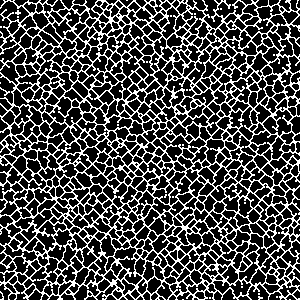
\includegraphics[width=0.5\textwidth]{./images/Time36-Process5.png}
\caption{
A still from simulation of process \ref{itm:6}, death-birth of the
fittest, at point $(5,3.5)$ on the bifurcation diagram and time 36. This is an
example of the distinct behavior of group 3 processes, as
they can tend towards steady states with neither strategy dominating
the lattice. This particular lattice was in approximately this
configuration from time 2 until the still was taken at time 36.
}
\label{fig:process6coexistence}
\end{figure}

\begin{figure}[h]
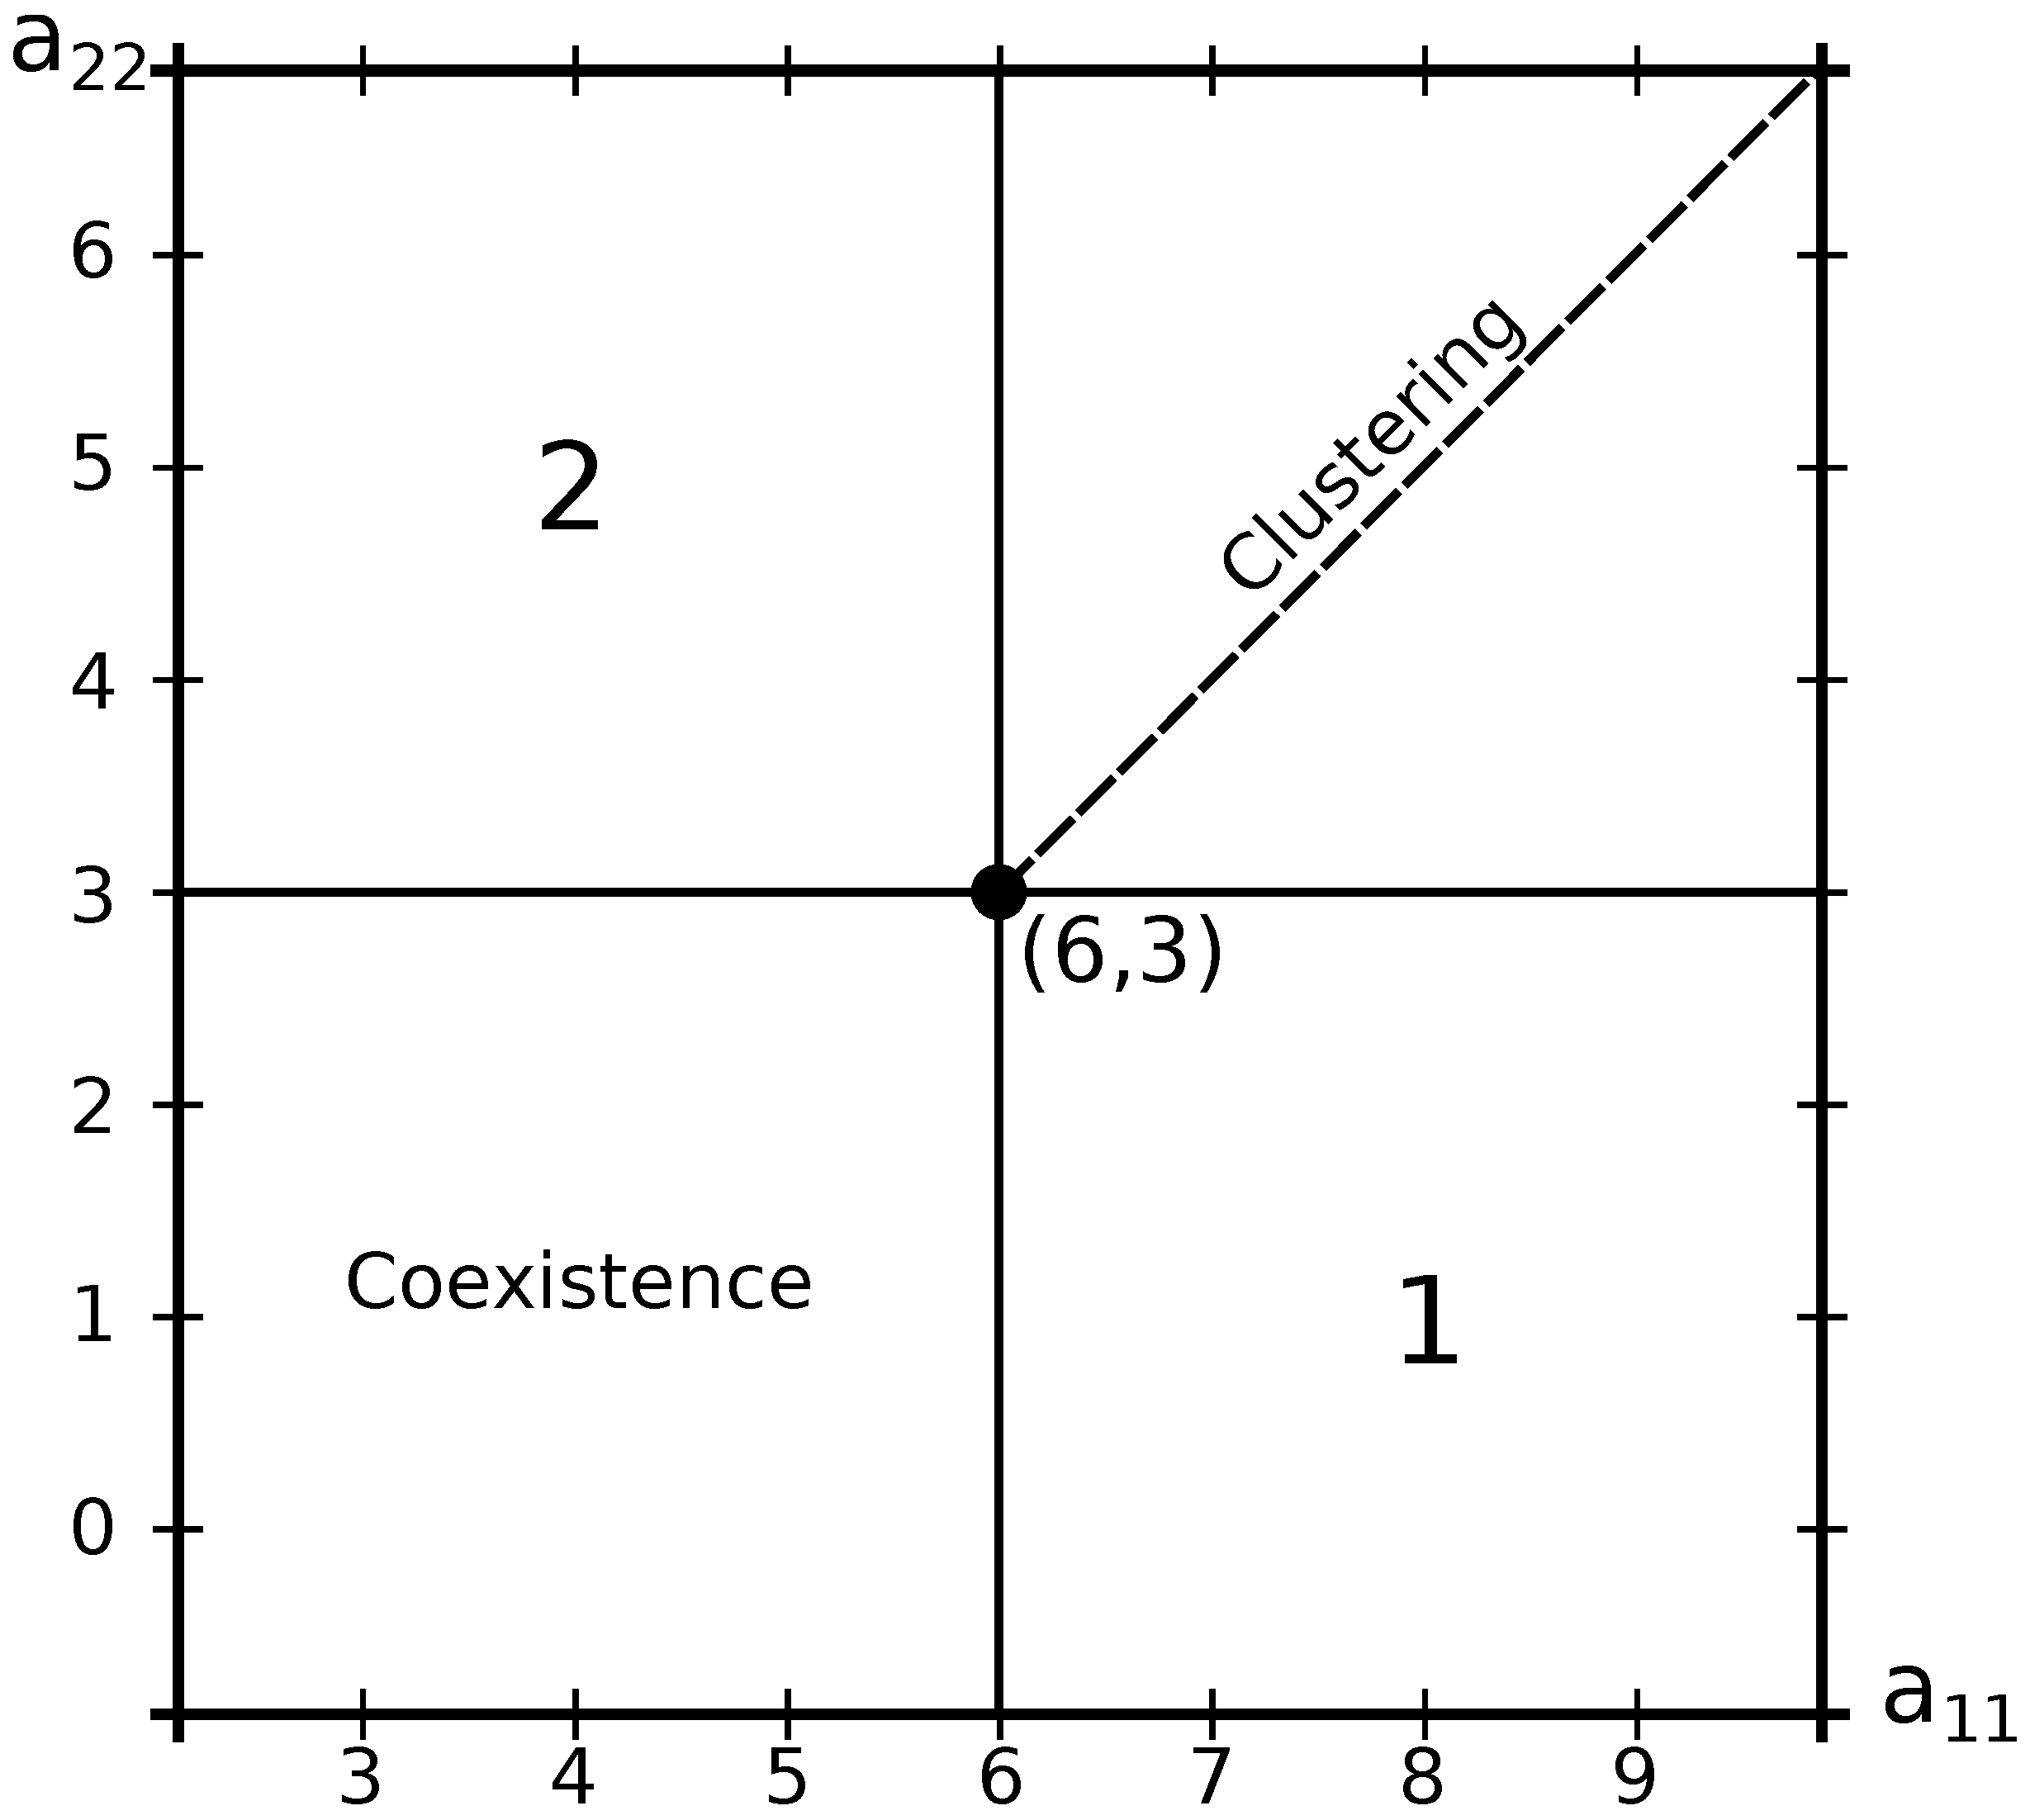
\includegraphics[width=0.5\textwidth]{./images/process_8_bifurcation_diagram.eps}
\caption{
A bifurcation diagram for process \ref{itm:8}.
}
\label{fig:process8diagram}
\end{figure}

It is finally worth examining process \ref{itm:8}, best response
dynamics. Its bifurcation diagram is found in Figure
\ref{fig:process8diagram}, which is exactly similar to Figure
\ref{fig:group1diagram} in quadrants I, II, and IV. Quadrant III,
however, is exactly the same as in the mean-field model; in every case
in the region, asymptotic behavior tends towards coexistence. Two
types of coexistence occurred: at the edges of the region and along a
continuation of the clustering line, we see ordinary coexistence. In
the rest of the region, though, behavior tended towards steady states
like those seen in Figure \ref{fig:process6coexistence}, though the
steady states in this process were much more chaotic.

\subsection{A few interesting cases}
Simulations of these processes are best viewed in real-time; their
stochastic and ever-changing nature limits the value of static
images. That said, there are a few cases that produce some interesting
stills, especially with process \ref{itm:1}, payoff affecting birth
and death. The first interesting cases offer a comparison between strong and weak
clustering, and they occurs in process \ref{itm:1} with the payoff
matrices
\[
    P_1 = \begin{pmatrix}
      1 & -1 \\
      -1 & 1
    \end{pmatrix}
\]
and
\[
    P_2 = \begin{pmatrix}
     1 & 0 \\
     0 & 1
   \end{pmatrix}
\]

In either payoff matrix, both strategies are selfish; $a_{11}$ and
$a_{22}$ are both equal to 1, which means that both strategies give
positive payoff to like players. In $P_1$, $a_{12} = a_{21} = -1$, which means that both players give negative payoff to
unlike players. In $P_2$, $a_{12} = a_{21} = 0$, which means that neither player affects the payoff of unlike players.

\begin{figure}[h]

\includegraphics[width=.4\textwidth]{./images/Time200-Process0.png}
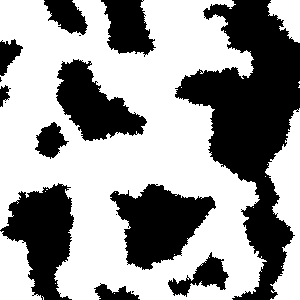
\includegraphics[width=.4\textwidth]{./images/Time200-Process0-1.png}
\caption{
  Two simulations of the payoff affecting birth and death process with two selfish strategies at time 200. On the left, both strategies deliver negative payoffs to opponents (payoff matrix $P_1$ above); on the right, zero payoff is given to opposing strategies (payoff matrix $P_2$ above).
}
\label{fig:proc1clustering}
\end{figure}

Figure \ref{fig:proc1clustering} shows two types of clustering
behavior. In the left-hand picture, the boundaries of each cluster are
smooth, because a site with the dominant strategy in the area will
eliminate nearby opponents, since $a_{ij}$ is negative for $i\neq
j$. On the right, we still have comparably-sized clusters, but the
boundaries aren't as smooth, because neither strategy is disadvantaged by
being adjacent to an opponent.

We can see an excellent example of coexistence behavior by making both
strategies in the payoff affecting birth and death process altruistic, with payoff matrix
\[
    P = \begin{pmatrix}
      -1 & 1 \\
      1 & -1
    \end{pmatrix}.
\]

\begin{figure}[h]

\includegraphics[width=.4\textwidth]{./images/Time10-Process0.png}

\includegraphics[width=.4\textwidth]{./images/Time1000-Process0.png}
\caption{A simulation of the payoff affecting birth and death process
  with two altruistic strategies at times 10 (left) and 200 (right).}
\label{fig:proc1coexistence}
\end{figure}

In Figure \ref{fig:proc1coexistence}, we see a configuration with weak
spatial correlations
across the lattice from the very beginning, and after a long time
nothing significant has changed. The lattice is under constant
variation the whole time, but there is no trend; the proportions of
white and black remain the same, as does the spatial distribution of
players on the lattice.

The nonlinear processes (\ref{itm:5}, \ref{itm:6}, \ref{itm:7}, and
\ref{itm:8}) can generate a few other interesting scenarios. With the
right initial configuration, the best response dynamics process
(process \ref{itm:8}) tends towards percolation. Because any site can
adopt either strategy at any time regardless of its surroundings, and
strategy 1 becomes optimal as long as one neighboring site employs
strategy 1, black clusters form in strict rectangles on the
lattice. With the payoff matrix
\[
    P = \begin{pmatrix}
      1.01 & 0 \\
      0 & 1
   \end{pmatrix}
\]
and a uniformly distributed initial configuration with one strategy 1
player for every five strategy 2 players, the outnumbered black sites
can still dominate the lattice. First, Figure \ref{fig:process8-1to6}
shows what happens if the ratio of black:white is too low (1:6 or
less). Here, we see a number of black clusters, but none is able to
grow large enough to overtake the lattice. However, with the right
ratio, we see a result like the series of images in Figure
\ref{fig:process8-1to5}, with a few small black clusters growing and
joining together to eventually dominate the lattice.

\begin{figure}[h]
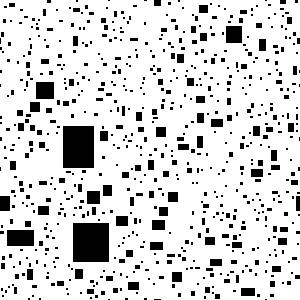
\includegraphics[width=.5\textwidth]{./images/Time41-Process7-cities.png}
\caption{
A simulation of the best response dynamics process with payoff matrix
set up for percolation, but with initial distribution ratio too low to
allow for percolation. This image is the steady state of the process;
after this point, the lattice did not change.
}
\label{fig:process8-1to6}
\end{figure}

\begin{figure}[h]
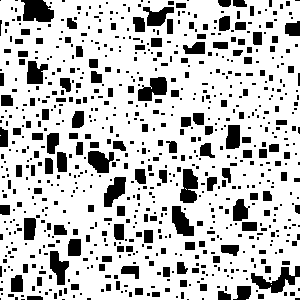
\includegraphics[width=.3\textwidth]{./images/Time4-Process7.png}
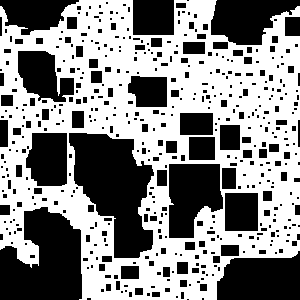
\includegraphics[width=.3\textwidth]{./images/Time25-Process7.png}
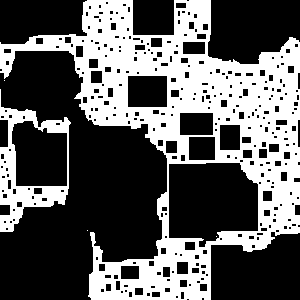
\includegraphics[width=.3\textwidth]{./images/Time41-Process7.png}
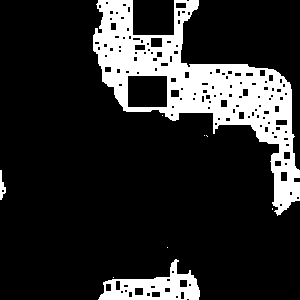
\includegraphics[width=.3\textwidth]{./images/Time61-Process7.png}
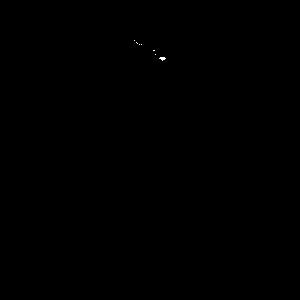
\includegraphics[width=.3\textwidth]{./images/Time95-Process7.png}
\caption{
A series of stills from simulation of the best response dynamics
process with payoff matrix and initial distribution set up for
percolation. From left to right, the stills were taken at times 4, 25,
41, 61, and 95. As time progresses, we see black clusters encroach upon
the larger white clusters and eventually overtake the lattice.
}
\label{fig:process8-1to5}
\end{figure}

We see a similar result with process \ref{itm:6}, death-birth of the
fittest. To cause percolation, we use the above payoff matrix, but with
$a_{11} = 1.5$. We also use an initial black:white ratio of 1:3. With
this arrangement, we see clusters forming diamonds rather than
rectangles. This behavior is seen in Figure
\ref{fig:process6percolation}.

\begin{figure}[h]
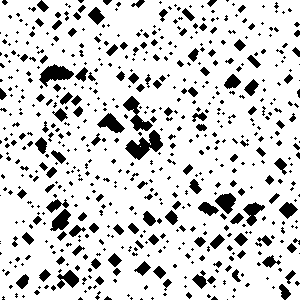
\includegraphics[width=.3\textwidth]{./images/Time2-Process5-1.png}
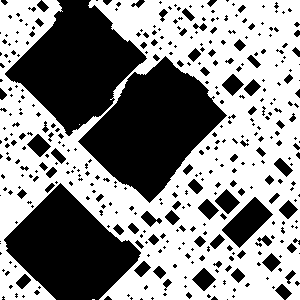
\includegraphics[width=.3\textwidth]{./images/Time40-Process5.png}
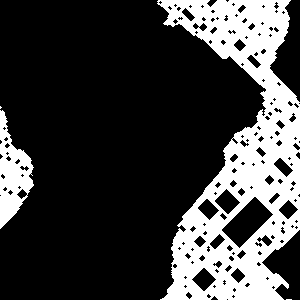
\includegraphics[width=.3\textwidth]{./images/Time65-Process5.png}
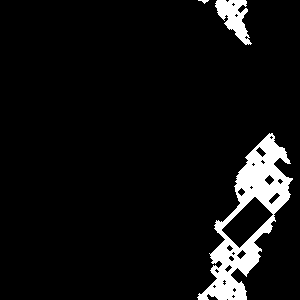
\includegraphics[width=.3\textwidth]{./images/Time79-Process5.png}
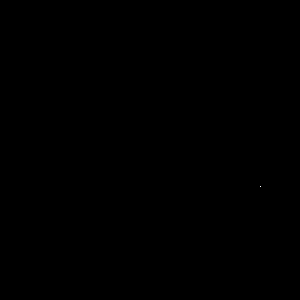
\includegraphics[width=.3\textwidth]{./images/Time89-Process5.png}
\caption{
A series of stills from simulation of the death-birth of the fittest
process with payoff matrix and initial distribution set up for
percolation. From left to right, the stills were taken at times 2, 40,
65, 79, and 89. As time progresses, we see black clusters encroach upon
the larger white clusters and eventually overtake the lattice.
}
\label{fig:process6percolation}
\end{figure}


\subsection{Cooperation in the Prisoner's Dilemma}

Perhaps the most life-affirming of the results from these spatial
processes comes from analysis of the prisoner's dilemma. In any given
prisoner's dilemma game, the optimal strategy for a rational player is
to defect; expected payoff is maximized if one chooses to betray her
accomplice. This follows in the mean-field model; for prisoner's
dilemma games (those with payoff coefficient order
$a_{21} > a_{11} > a_{22} > a_{12}$), the defector strategy (strategy
2 in our setup) dominates the population. This is verified when we
consider what region of the bifurcation diagram represents prisoner's
dilemma games. As shown in \ref{fig:gametypesdiagram}, the coefficient
order of the prisoner's dilemma puts it in quadrant II (as
$a_{21}>a_{11}$ and $a_{22}>a_{12}$) and under the line $a_{22} =
a_{11}$ (as $a_{11}>a_{22}$). In the bifurcation diagram for the
replicator equation, this region is entirely contained in the region
in which strategy 2, the defector strategy, wins. This result even
holds for the spatial model with group 1 processes, as shown in
Figure \ref{fig:group1withpd}.

\begin{figure}[h]
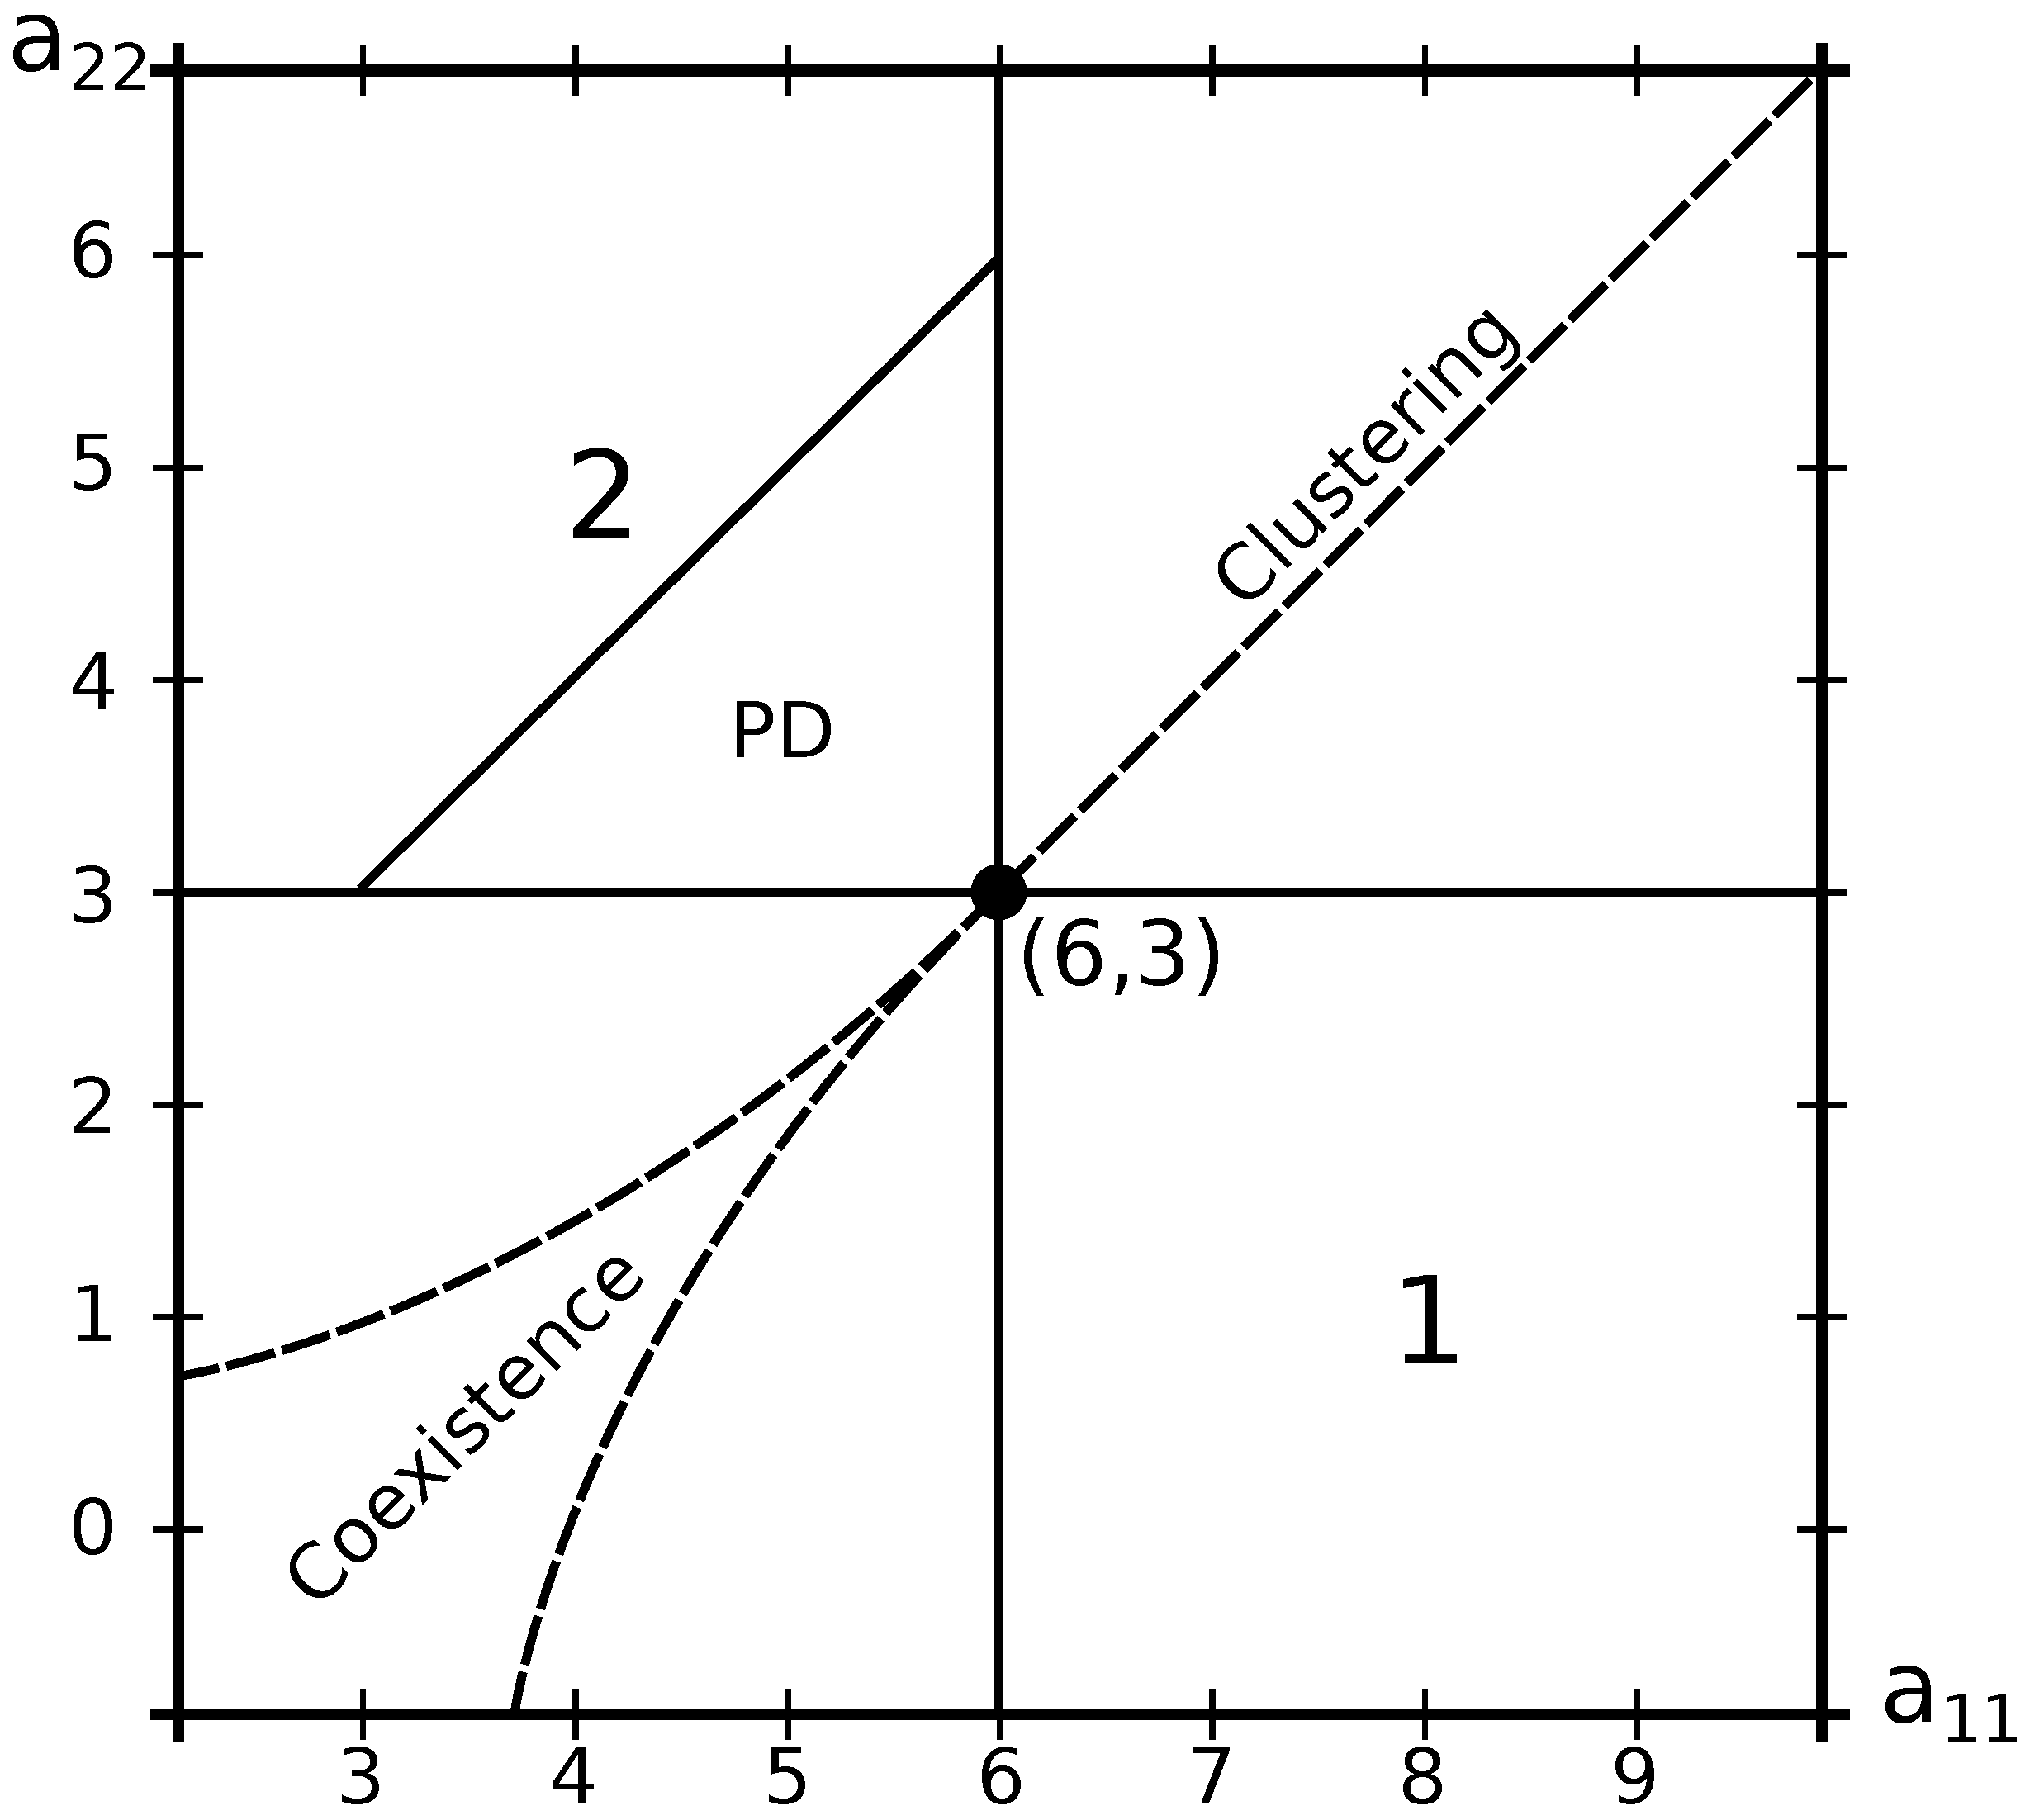
\includegraphics[width=.5\textwidth]{./images/group_1_bifurcation_diagram_w_PD.eps}
\caption{A bifurcation diagram for group 1 processes showing that
  strategy 2 dominates the lattice in the prisoner's dilemma region.}
\label{fig:group1withpd}
\end{figure}

We see a different result, however, for groups 2 and 3. As shown in
Figure \ref{fig:groups2and3withpd}, the curves along which clustering
occurs cut the prisoner's dilemma region into pieces. Below these curves,
strategy 1, the cooperator strategy, dominates the lattice.

\begin{figure}[h]
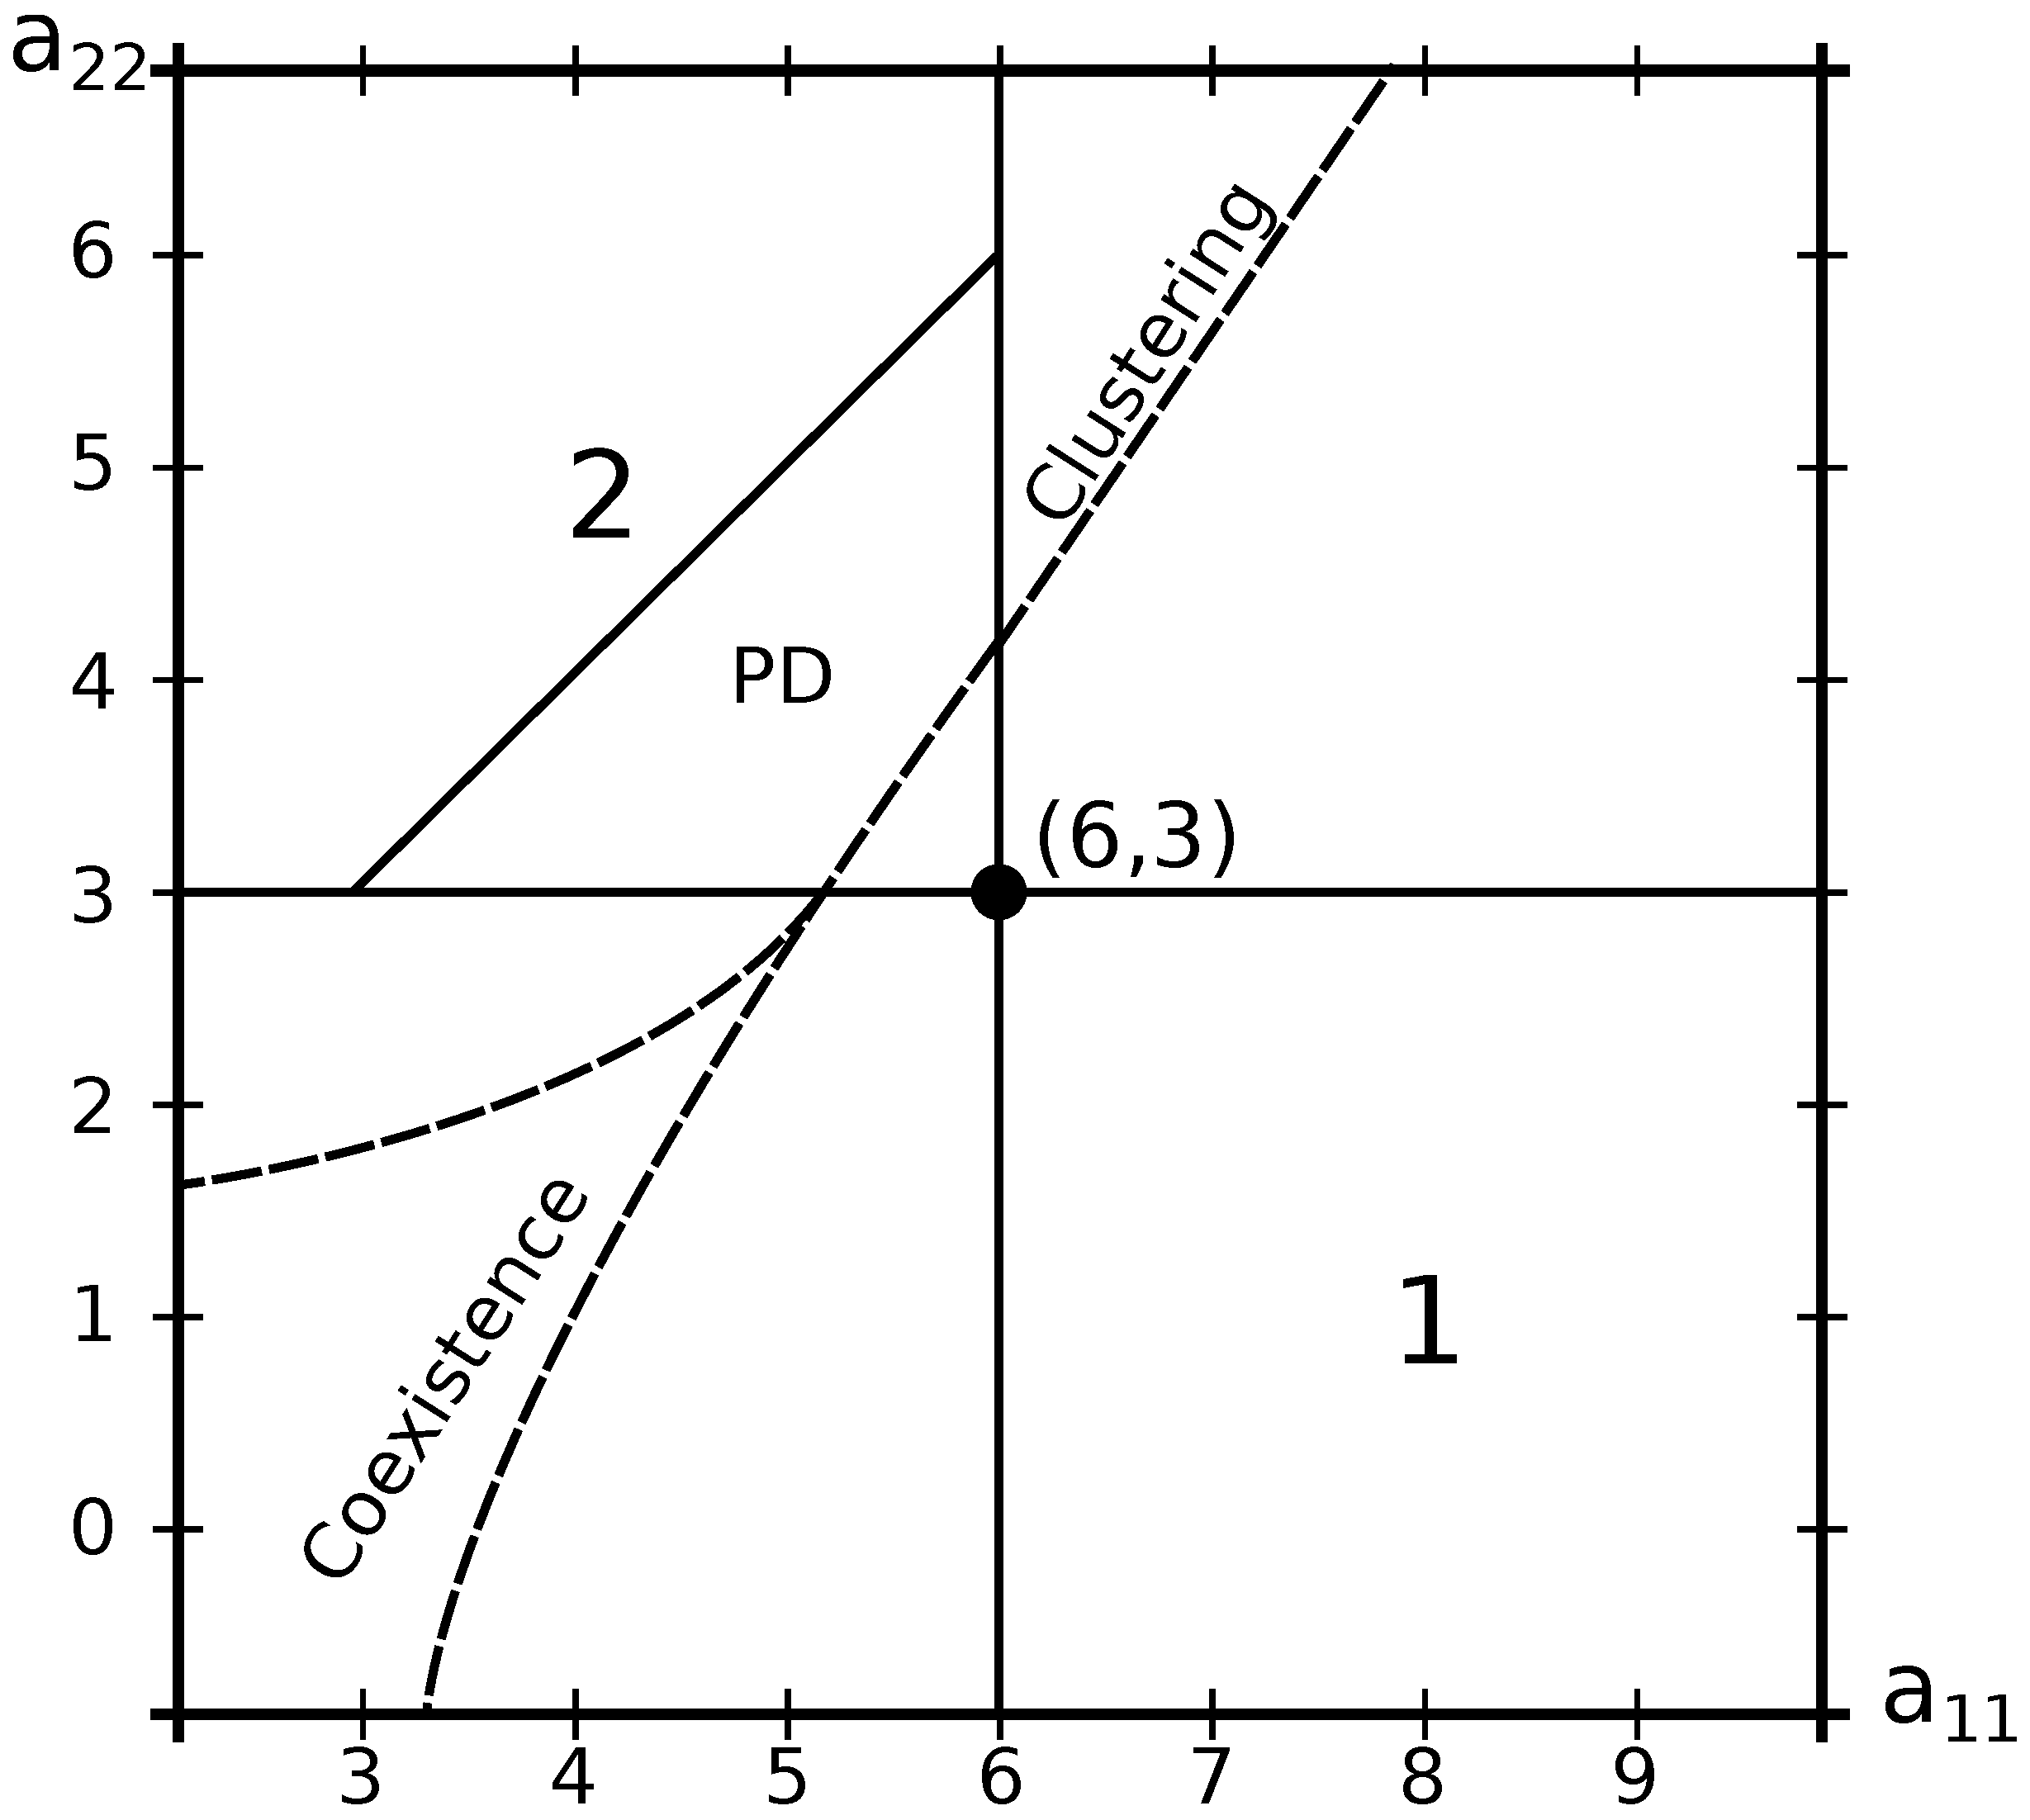
\includegraphics[width=.5\textwidth]{./images/group_2_bifurcation_diagram_w_PD.eps}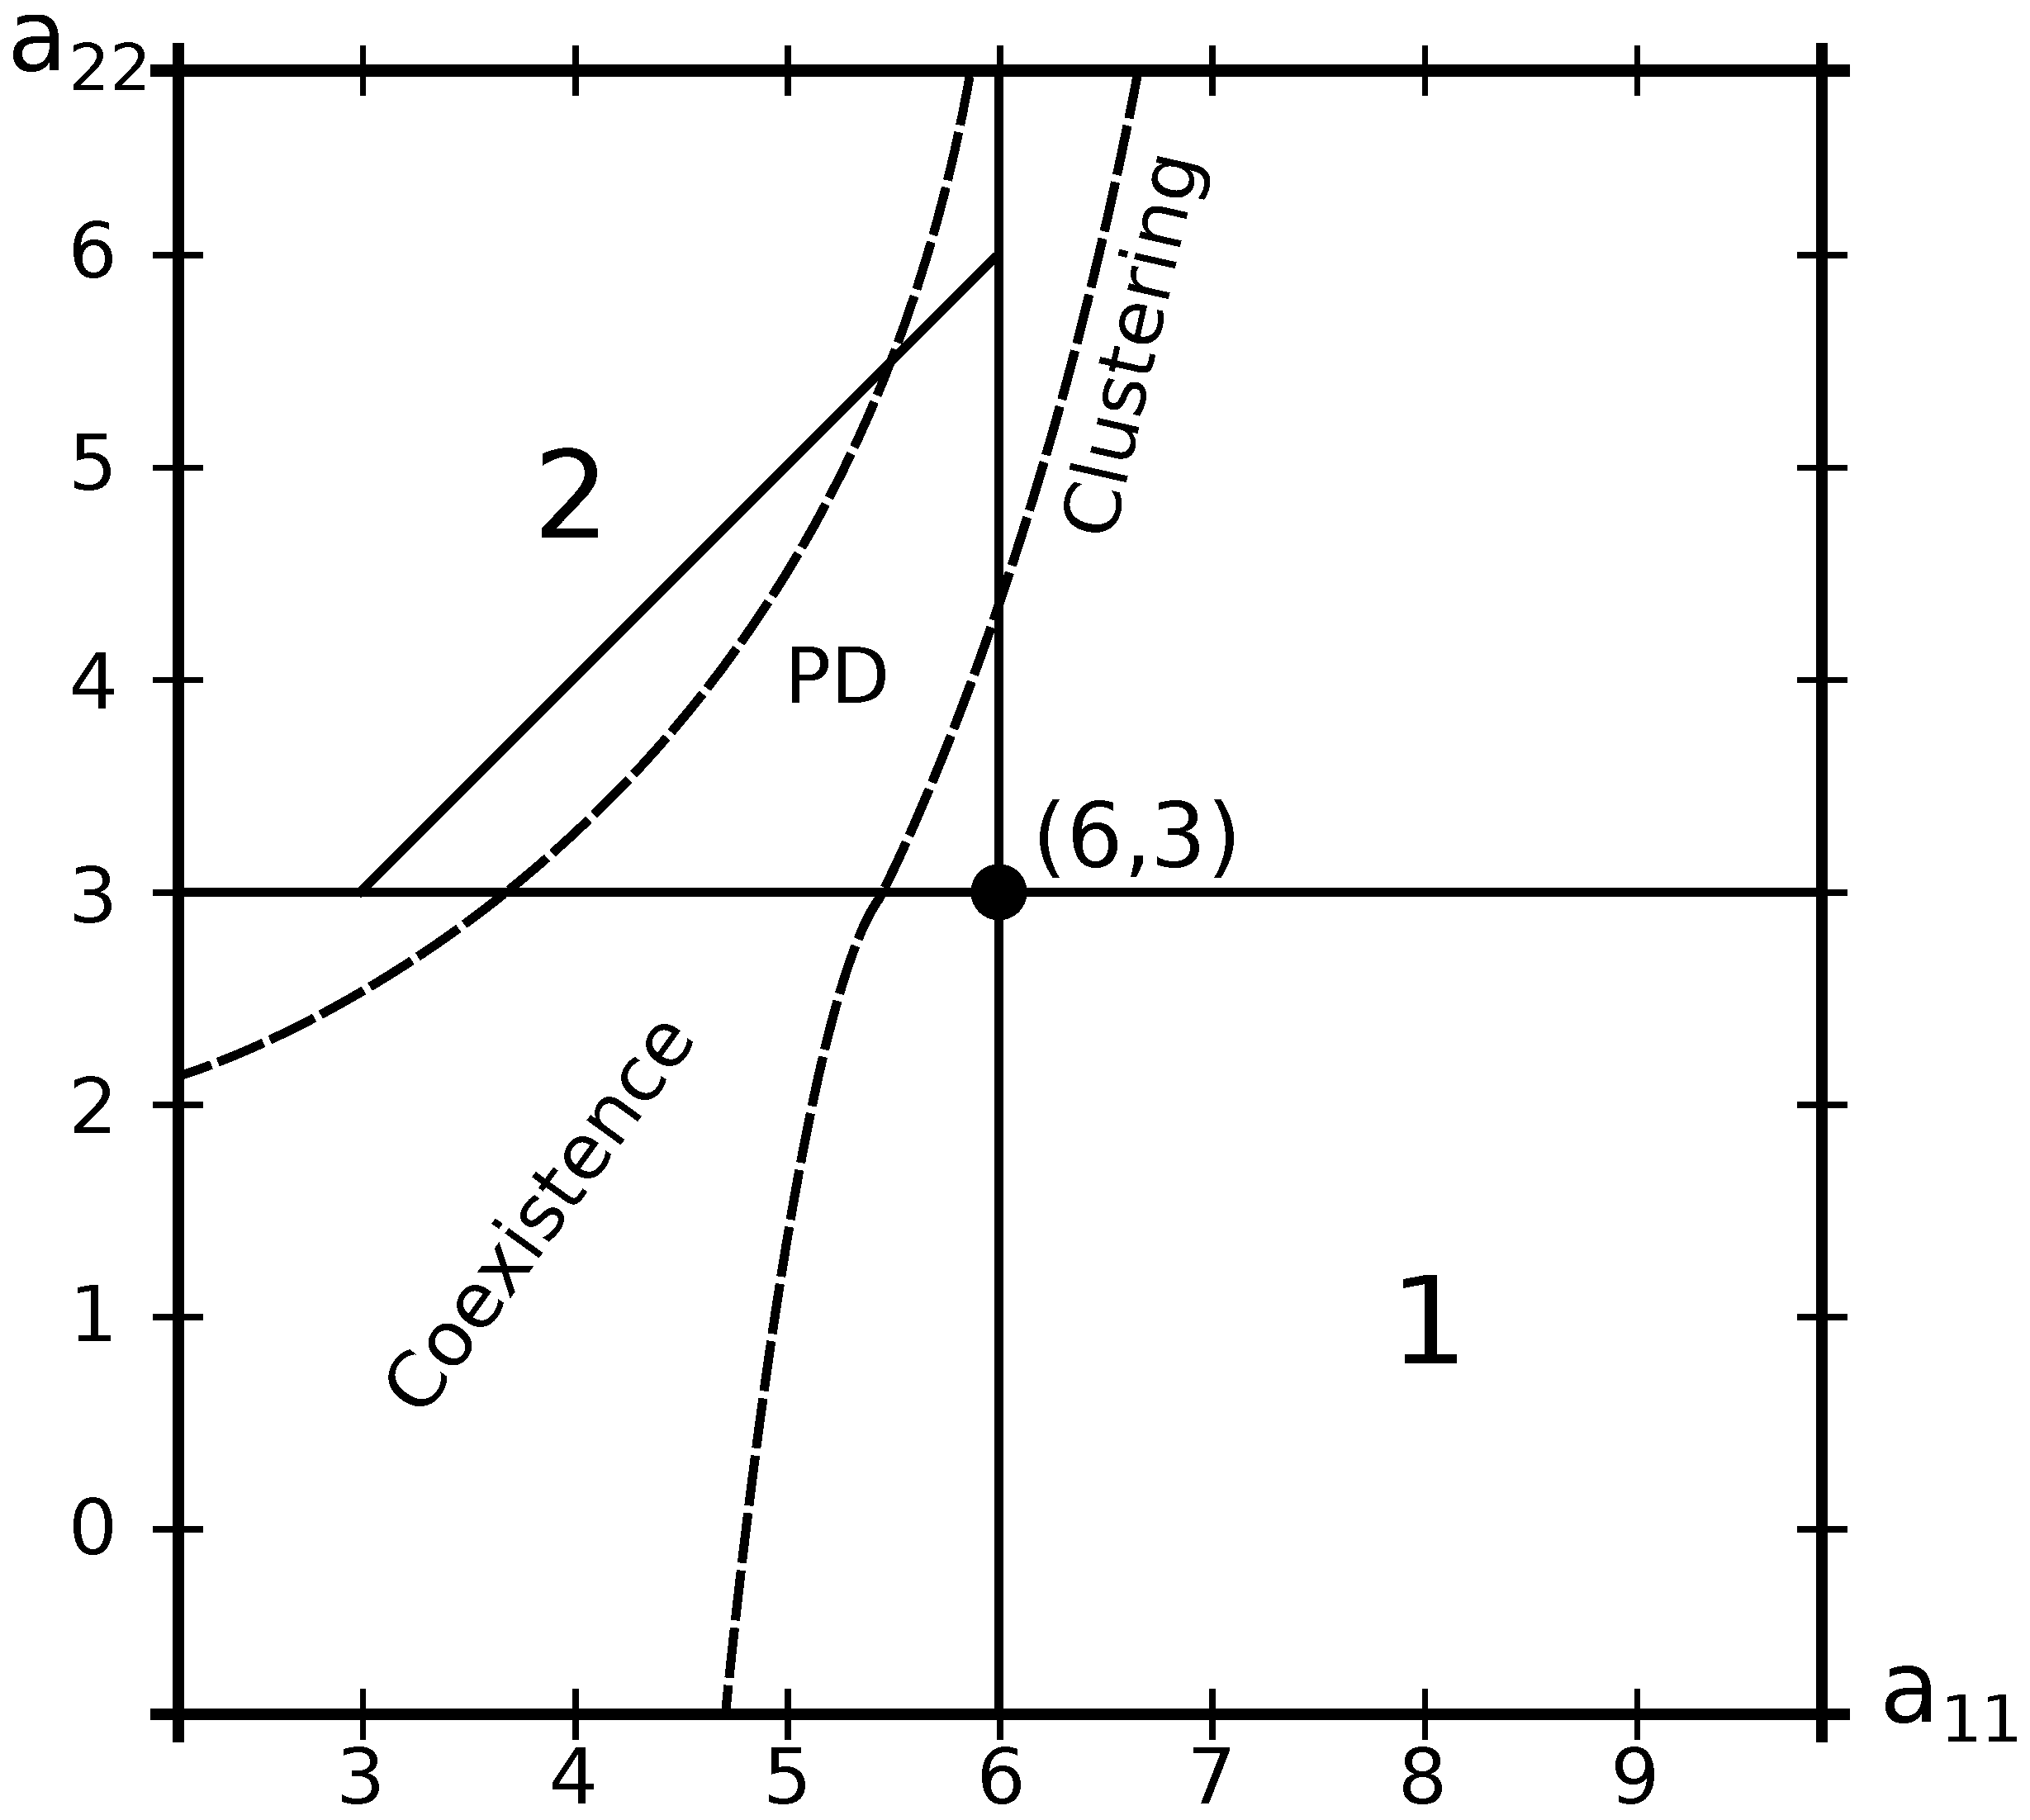
\includegraphics[width=.5\textwidth]{./images/group_3_bifurcation_diagram_w_PD.eps}
\caption{A bifurcation diagram for groups 2 and 3 processes showing
  that strategy 1 dominates the lattice for some games in the
  prisoner's dilemma region.}
\label{fig:groups2and3withpd}
\end{figure}

We have not proven these results analytically, as the bifurcation
diagrams are constructed only from simulations. We can, however, prove
this result in an extremely special case. On a one-dimensional lattice
with two strategies using process \ref{itm:3}, the death-birth process,
and with a specific initial configuration, there is a region of the
prisoner's dilemma triangle in which cooperation is the long-term
dominating strategy. This initial condition is pictured in Figure
\ref{fig:initialconfiguration}; all strategy 1 players are to the left
of some site $X_t$, while all strategy 2 players are at $X_t$ and to
the right of $X_t$. With this configuration, it is easy to see that
the only way in which the lattice can change is if the interface (that
is, the leftmost white site) moves. This can only occur only if either $X_t$ or
$X_t-1$ is selected to die and the selected site is replaced by a
player of the opposite strategy. The rates at which these two events occur
depend upon the payoffs for $X_t$, $X_t-1$, $X_t-2$, and $X_t+1$,
which follow:
\begin{align*}
  \phi_{X_t-2} &= 2a_{11} \\
  \phi_{X_t-1} &= a_{11} + a_{12} \\
  \phi_{X_t} &= a_{22} + a_{21} \\
  \phi_{X_t+1} &= 2a_{22}.
\end{align*}

\begin{figure}[h]
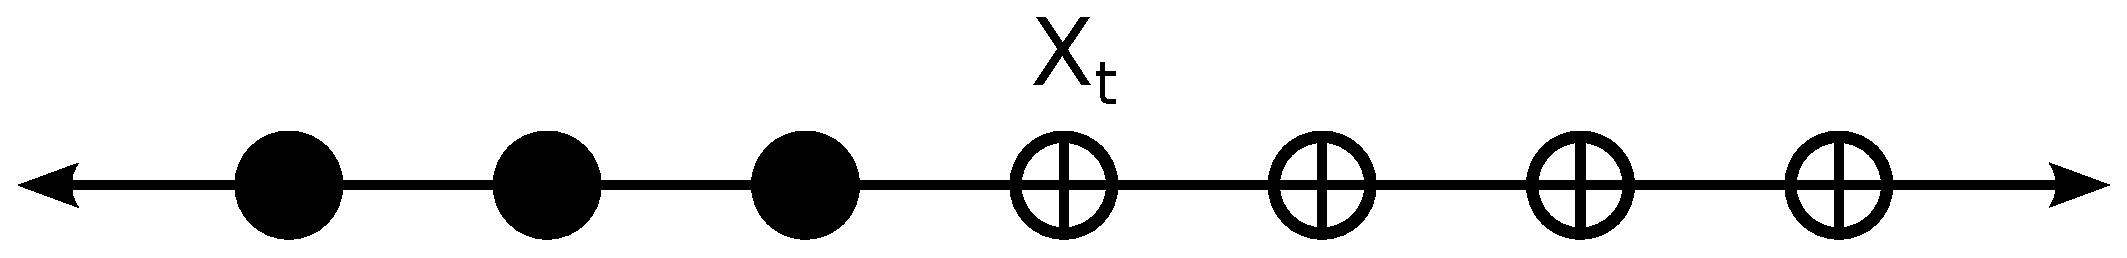
\includegraphics[width=0.9\textwidth]{./images/1dInitialConfig_w_label.eps}
\caption{A special-case initial configuration for a one-dimensional
  lattice. Sites colored black hold players of strategy 1, while sites
colored white hold players of strategy 2.}
\label{fig:initialconfiguration}
\end{figure}

From the definition of process 3, we have that each site dies at rate
1. From Lemma \ref{lem:minofexponentials}, we know that this means
that each site is equally likely to be selected for update. This means
that $X_t$ and $X_t-1$ are equally likely to be selected to die at any
step. If $X_t-1$ is selected, the interface will move if and only if
the player at that site is replaced by a strategy 2 (white)
player. This occurs with probability
\[
    \frac{\phi_{X_t}}{\phi_{X_t} + \phi_{X_t-2}}
\]
and will cause the interface to move one site to the left. Similarly,
if $X_t$ is selected, the interface will move if and only if the
player at that site is replaced by a strategy 1 (black) player. This
occurs with probability
\[
    \frac{\phi_{X_t-1}}{\phi_{X_t-1} + \phi_{X_t+1}}
\]
and will cause the interface to move one site to the right. Thus, we
have the interface moving according to a continuous-time random walk
with the above rates. Because this random walk is one-dimensional, we
can quickly see that strategy 1 will dominate the lattice if movement
to the right is more likely, while strategy 2 will dominate if
movement to the left is more likely. Thus, we are interested in the
conditions for a symmetric random walk, which clearly occurs when
\[
    \frac{\phi_{X_t}}{\phi_{X_t} + \phi_{X_t-2}} = \frac{\phi_{X_t-1}}{\phi_{X_t-1} + \phi_{X_t+1}}.
\]

In terms of payoff coefficients, this becomes
\[
    \frac{a_{22}+a_{21}}{a_{22}+a_{21} + 2a_{11}} =
    \frac{a_{11}+a_{12}}{a_{11} + a_{12} + 2a_{22}}.
\]
The curve defined by this equation is shown in Figure
\ref{fig:pddiagram}, below. As predicted by the simulated results, this
curve cuts the prisoner's dilemma region into two parts, and in the
lower part, cooperators dominate the lattice in the long-run.

\begin{figure}[h]
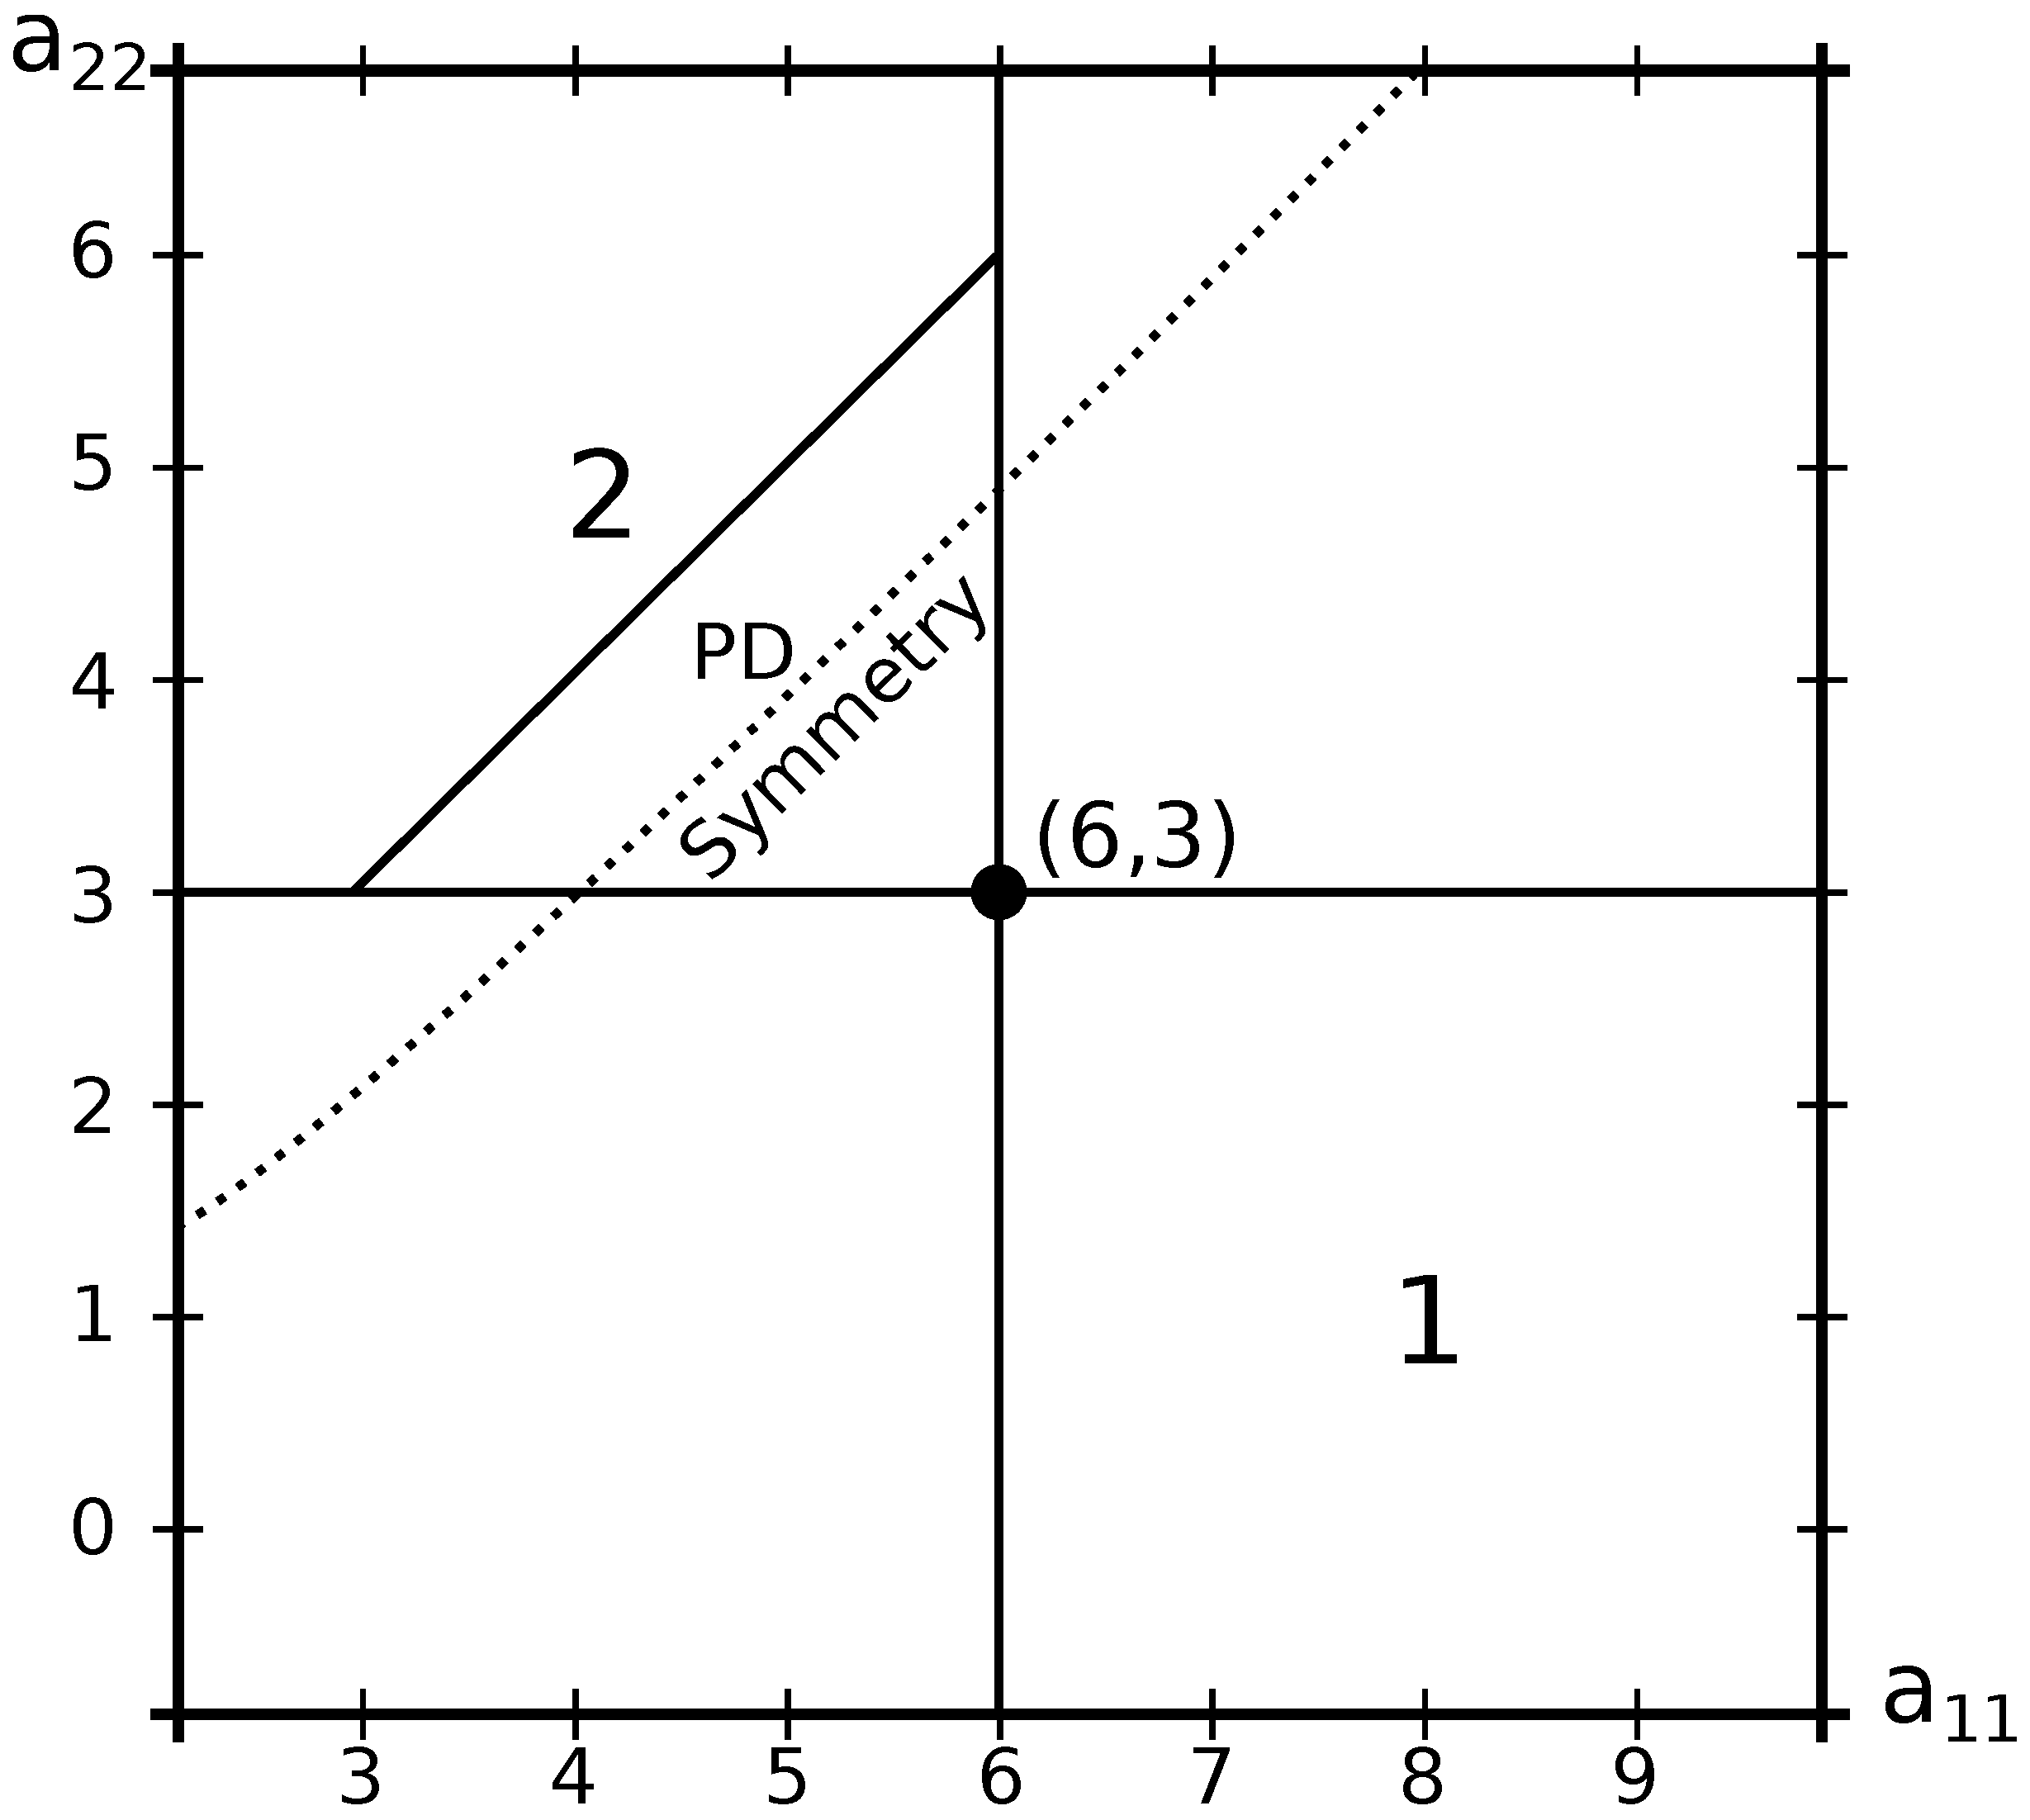
\includegraphics[width=0.7\textwidth]{./images/1d_pd_plot.eps}
\caption{A bifurcation diagram for group 2 processes with the curve
  along which the random walk of the one-dimensional interface is
  symmetrical.}
\label{fig:pddiagram}
\end{figure}

\section{Conclusions}

This result is extremely satisfying, because it more accurately
reflects the ways in which humans actually behave than the prisoner's
dilemma does ordinarily. The prisoner's dilemma is often used as a
model for human interaction because it accurately represents many
competitive situations, but the conclusion that defection is optimal
is distressing -- humans have come to dominate the globe not by
betraying one another, but by cooperating. Spatial consideration,
though, seems to help alleviate this inconsistency by showing that, at
least in some cases, cooperation is in fact the best option.


%% \section{Appendix}
%% \subsection{\texttt{Lattice.java}}
%% \lstinputlisting{./code/Lattice.java}

%% \subsection{\texttt{SimulatorApplet.java}}
%% \lstinputlisting{./code/SimulatorApplet.java}

\newpage

\bibliographystyle{plain}{}
\bibliography{bibliography}

\end{document}
